% PLDI 2027 review paper. Compile main.tex with pdfLaTeX and BibTeX.
% Official format: https://pldi27.sigplan.org/track/pldi-2027-papers
\documentclass[acmsmall,screen,review,anonymous,nonacm]{acmart}
\citestyle{acmnumeric}
\settopmatter{printacmref=false}
\usepackage{amsmath}
\usepackage{array}
\usepackage{tikz}
\usetikzlibrary{arrows.meta,positioning,fit,calc,backgrounds,shapes.geometric}
\usepackage{xurl}
\urlstyle{same}
% Shared palette follows the supplied high-assurance diagram.
% Pastel fills are separate from saturated outlines; labels preserve grayscale meaning.
\definecolor{scpBlue}{RGB}{31,78,121}
\definecolor{scpGreen}{RGB}{0,140,64}
\definecolor{scpRed}{RGB}{192,0,0}
\definecolor{scpGray}{RGB}{94,102,112}
\definecolor{scpBlueFill}{RGB}{221,235,247}
\definecolor{scpGreenFill}{RGB}{227,243,209}
\definecolor{scpRedFill}{RGB}{255,232,232}
\definecolor{scpGrayFill}{RGB}{241,238,235}
\definecolor{scpYellowFill}{RGB}{255,242,204}
\definecolor{scpPurple}{RGB}{112,48,160}
\tikzset{
  scpProposal/.style={draw=scpBlue,fill=scpBlueFill,text=black},
  scpCheck/.style={draw=scpGreen,fill=scpGreenFill,text=black},
  scpOpen/.style={draw=scpRed,fill=scpRedFill,text=black,dashed},
  scpRecord/.style={draw=scpGray,fill=scpGrayFill,text=black},
  scpDataFlow/.style={draw=scpBlue},
  scpCheckFlow/.style={draw=scpGreen},
  scpRepairFlow/.style={draw=scpRed,dashed},
  scpRecordFlow/.style={draw=scpGray}
}

% Pseudocode uses algorithm2e with numbered lines and block guides.
\RequirePackage[ruled,vlined,linesnumbered]{algorithm2e}
\DontPrintSemicolon
\SetCommentSty{textnormal}
\SetArgSty{textnormal}
\SetAlFnt{\small}
\SetAlCapFnt{\small\bfseries}
\SetAlCapNameFnt{\small\bfseries}
\SetAlgoCaptionSeparator{.}
\SetAlgoNlRelativeSize{-1}
\SetKwInput{KwIn}{Input}
\SetKwInput{KwOut}{Output}
\newcommand{\scpPhase}[1]{\textbf{#1}\;}
\newcommand{\scpStatus}[1]{\textnormal{\textsc{#1}}}

\newcommand{\papersection}[2]{\ref{#1}}
\newcommand{\paperfigure}[2]{\ref{#1}}
\newcommand{\workbench}{SCP Workbench}
\hypersetup{pdfauthor={},pdftitle={Rule Evolution for Formally Verifiable seL4 Applications}}
\title[Rule Evolution for Verifiable seL4 Applications]{Rule Evolution for Formally Verifiable seL4 Applications}
\subtitle{From Requirements to Execution with the Accountable Neuro-Symbolic SCP Workbench}
\author{Anonymous Author(s)}

\begin{document}
\begin{abstract}
Repairing a system model can invalidate the proofs, tests, and approvals for its generated code. The Spec--Code--Proof (SCP) Workbench supports model-based engineering from reviewed English requirements and design context through SysML v2 models and contracts, code generation and repair, formal checks, and seL4 execution. Supervised rule evolution turns tool diagnostics and reviewed repairs into versioned guidance with applicability conditions and required checks. Workers reuse selected rule files in isolated workspaces. The controller binds checks and approvals to reviewed revisions and retains costs across authorized repairs.

Held out of Monitor training, Producer/\allowbreak{}Consumer started from English and existing rulebooks with zero supplied target-model lines in the reported dispatch. Three successful build inventories total 26,758 source lines, including generated code, tests, and bundled support. In a later common-input Simple Network Guard (SNG) pair, the arm receiving a 66-entry rule bundle passed five model checks at 346,224 measured tokens. The baseline stopped at its repair limit after 388,726 tokens. The guided continuation delivered a 13,133-line build with 32 Verus proof units discharged under recorded premises and passing Rust and JVM tests. Source and image fingerprints link checked component code and the built Microkit image to 20.033 seconds of QEMU observation after readiness.

\end{abstract}
\ccsdesc[500]{Software and its engineering~Formal methods}
\ccsdesc[300]{Computing methodologies~Artificial intelligence}
\keywords{supervised meta-learning, formal verification, neuro-symbolic engineering, seL4, scoped attestation, model-based systems engineering}
\maketitle
\hypersetup{pdfauthor={},pdftitle={Rule Evolution for Formally Verifiable seL4 Applications}}

\section{Introduction}
\label{sec:introduction}

Behrang et al.~\cite{behrang2025drfix} combine language models with program analysis to repair data races. Lee and Heo~\cite{lee2026expecto} derive formal test oracles from text to expose behavioral bugs. In embedded systems, changing a model contract can invalidate generated code, proofs, tests, and the approval under which they ran. An agent can use tool diagnostics to propose a repair. The engineer needs to know which obligations were checked for the revision, which assumptions the checks used, and who authorized the next step. These questions recur when a later system reuses lessons from an earlier repair.

We present the Spec--Code--Proof (SCP) Workbench, a neuro-symbolic system for model-based systems engineering (MBSE). It constructs SysML v2 models with GUMBO contracts from reviewed English and design context. The controller coordinates HAMR generation for Slang and Rust, checks with Logika and Verus, and builds and runs a seL4 application using Microkit (Figure~\ref{fig:engineering-stack})~\cite{inspectaProject,hardin2025dasc,hamrTutorials2026}. The controller supplies selected rule versions to workers in fresh workspaces. Acceptance requires evidence and approval for the current revision, assumptions, and scope.

Tahat et al.~\cite{tahat2026scp} used reusable rules and HAMR/Logika checks to generate and repair GUMBO contracts within supplied Isolette models. The companion demonstration supplied the Slang/Scala application logic~\cite{inspecta_repo}. The \workbench{} extends this approach to constructing target models, checking the generated Rust and Slang implementations, and building and observing a runnable image. Its campaign record connects each stage to the revision it assessed and the decision that authorized continuation. Table~\ref{tab:related-work} compares the starting artifacts and outcomes of related systems.

Our contributions are the following.
\begin{enumerate}
\item \textbf{Executable engineering workflow.} A controller coordinates model proposals, generation, repairs, proofs, tests, builds, and runtime observation. It preserves earlier outcomes and cumulative expenditure across authorized continuations (Figure~\ref{fig:control-handoff}).
\item \textbf{Budgeted supervised meta-learning.} Engineering attempts and tool diagnostics yield rules with applicability conditions, required checks, earlier versions, and supporting evidence. A declared file handoff carries selected rule versions into a new workspace, where subsequent attempts can refine them (Figures~\ref{fig:handoff} and~\ref{fig:evolution}).
\item \textbf{Scoped review and attestation.} Engineers delegate actions within approved limits and decide changes to assumptions, scope, and release. The protocol binds decisions to artifact fingerprints and evidence, and supports signed export for checking under an independently supplied policy (Figure~\ref{fig:attestation}).
\end{enumerate}

The evaluation follows reuse across the Isolette Regulator holdout, Producer/\allowbreak{}Consumer, and the Simple Network Guard (SNG). Three successful build inventories contain 26,758 source lines (Table~\ref{tab:source-line-counts}). In the later SNG comparison, the candidate receiving the 66-entry bundle passed all five model checks on shared task inputs. The controller rejected a proposal to delete an existing test and preserved its cost. The final Gate and Filter proof-input fingerprints match the corresponding Rust files in the build and observation inventories, and the loader digest identifies the image observed in QEMU~\cite{sngFinalReport2026}.

\section{Background and Running Example}
\label{sec:background}

\subsection{Engineering and Verification Tools}
SysML v2 models structure and interfaces~\cite{sysmlv2_omg}. GUMBO adds behavioral contracts~\cite{gumbo}. An \emph{assume--guarantee contract} $(A,G)$ requires $G$ when its assumptions $A$ hold. An \emph{obligation} is a property to establish under stated assumptions. HAMR derives infrastructure and contracts for Slang and Rust~\cite{hamr}. Logika checks Slang and connection obligations. Its configured integration checks use the cvc5 satisfiability modulo theories (SMT) solver~\cite{hallerstede2025logika,scpCheckpoint}. Verus checks Rust obligations and uses an SMT backend such as Z3~\cite{verusGuide}. GumboX derives executable checks, and Microkit provides a seL4 image target~\cite{hamrGumboxRust,hamr-sel4}.

\begin{figure}[t]
\centering
\resizebox{\textwidth}{!}{% Native-width PACMPL adaptation of the agent/toolchain illustration.
% The nested target artifacts and separate upstream/application proof targets
% retain the source figure's meaning; arrows describe available capabilities.
\begingroup
\hyphenpenalty=10000
\newcommand{\scpRobot}{%
  \tikz[x=.78pt,y=.78pt,baseline=-1.5pt,draw=scpBlue,line width=.45pt]{%
    \draw[rounded corners=.8pt,fill=scpBlueFill] (0,0) rectangle (9,6);
    \draw (0,2)--(-1.2,2) (9,2)--(10.2,2) (4.5,6)--(4.5,8);
    \fill[scpBlue] (4.5,8) circle (.60) (2.6,3.8) circle (.52) (6.4,3.8) circle (.52);
    \draw (3.2,1.8)--(5.8,1.8);
  }%
}
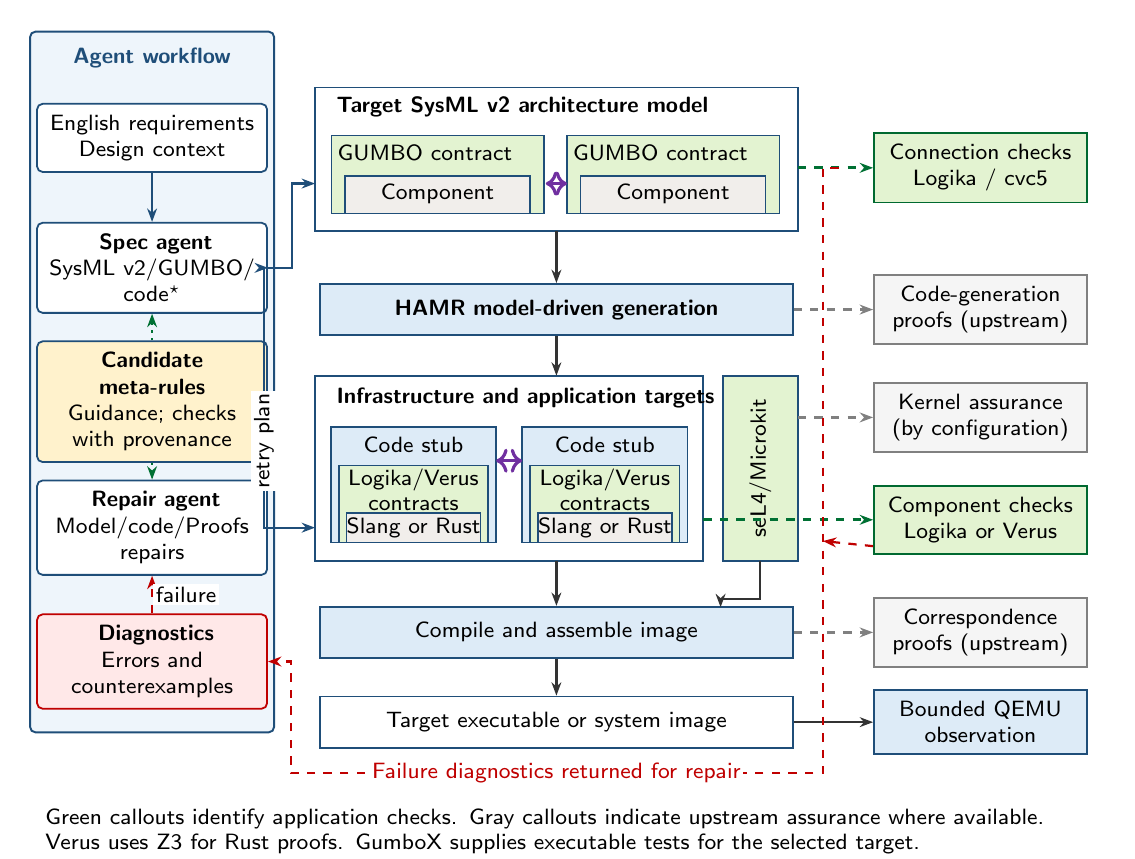
\begin{tikzpicture}[
 x=1cm,y=1cm,
 font=\sffamily\fontsize{8.2}{9.5}\selectfont,
 panel/.style={draw=scpBlue,line width=.7pt,rounded corners=2pt,fill=scpBlueFill!50},
 agent/.style={draw=scpBlue,line width=.65pt,rounded corners=2pt,fill=white,
   text width=2.64cm,align=center,inner sep=4pt,minimum height=.70cm},
 layer/.style={draw=scpBlue,line width=.65pt,fill=scpBlueFill,
   text width=5.72cm,align=center,inner sep=4pt,minimum height=.65cm},
 proof/.style={draw=scpGreen!75!black,line width=.7pt,fill=scpGreenFill,
   text width=2.42cm,align=center,inner sep=4pt,minimum height=.70cm},
 upstream/.style={proof,draw=black!50,fill=black!4},
 flow/.style={-{Stealth[length=1.7mm,width=1.25mm]},line width=.8pt,draw=black!80},
 proposal/.style={flow,draw=scpBlue},
 repair/.style={flow,draw=scpRed,dashed},
 check/.style={flow,draw=scpGreen!80!black,dashed,line width=1pt},
 prior/.style={check,draw=black!50},
 label/.style={fill=white,inner sep=1pt,align=center,font=\sffamily\fontsize{7.6}{8.7}\selectfont}
]
\path[use as bounding box] (0,-.70) rectangle (13.70,9.50);
% Agent workflow, distinct from the target system's artifacts.
\draw[panel] (.03,.55) rectangle (3.13,9.45);
\node[align=center,font=\sffamily\bfseries\fontsize{8.5}{9.8}\selectfont,text=scpBlue]
 at (1.58,9.12) {Agent workflow};
\node[agent] (requirements) at (1.58,8.10) {English requirements\\Design context};
\node[agent] (specagent) at (1.58,6.45) {\scpRobot\ \textbf{Spec agent}\\SysML v2/GUMBO/\\code\(^{\star}\)};
\node[agent,fill=scpYellowFill] (rules) at (1.58,4.75)
 {\textbf{Candidate meta-rules}\\Guidance; checks\\with provenance};
\node[agent] (repairagent) at (1.58,3.15)
 {\scpRobot\ \textbf{Repair agent}\\Model/code/Proofs\\repairs};
\node[agent,draw=scpRed,fill=scpRedFill] (diagnostics) at (1.58,1.45)
 {\scpRobot\ \textbf{Diagnostics}\\Errors and\\counterexamples};
\draw[proposal] (requirements.south) -- (specagent.north);
\draw[flow,draw=scpGreen!80!black,dotted] (rules.north) -- (specagent.south);
\draw[flow,draw=scpGreen!80!black,dotted] (rules.south) -- (repairagent.north);
\draw[repair] (diagnostics.north) -- node[label,right]{failure} (repairagent.south);
\draw[proposal] (repairagent.east) -- (3.00,3.15) -- (3.00,6.45) -- (specagent.east);
\draw[proposal] (repairagent.east) -- (3.65,3.15);
\node[label,rotate=90] at (3.00,4.25) {retry plan};
% Target architecture: two components and their contracts.
\draw[draw=scpBlue,line width=.7pt,fill=white] (3.65,6.92) rectangle (9.78,8.74);
\node[anchor=west,font=\sffamily\bfseries\fontsize{8.2}{9.5}\selectfont]
 at (3.80,8.49) {Target SysML v2 architecture model};
\foreach \x in {3.86,6.85}{
 \draw[draw=scpBlue,line width=.6pt,fill=scpGreenFill] (\x,7.14) rectangle +(2.70,.99);
 \node[anchor=north west,inner sep=2pt] at (\x,8.08) {GUMBO contract};
 \draw[draw=scpBlue,line width=.6pt,fill=scpGrayFill] (\x+.17,7.14) rectangle +(2.35,.48);
 \node at (\x+1.345,7.39) {Component};
}
\draw[<->,draw=scpPurple,line width=1.15pt] (6.58,7.52) -- (6.85,7.52);
\draw[proposal] (specagent.east) -- (3.36,6.45) -- (3.36,7.52) -- (3.65,7.52);
% Generation and implementation layers.
\node[layer] (generation) at (6.715,5.92) {\textbf{HAMR model-driven generation}};
\draw[flow] (6.715,6.92) -- (generation.north);
\draw[draw=scpBlue,line width=.7pt,fill=white] (3.65,2.73) rectangle (8.58,5.08);
\node[anchor=west,font=\sffamily\bfseries\fontsize{8.2}{9.5}\selectfont]
 at (3.80,4.80) {Infrastructure and application targets};
\foreach \x in {3.85,6.28}{
 \draw[draw=scpBlue,line width=.6pt,fill=scpBlueFill] (\x,2.96) rectangle +(2.10,1.47);
 \node[align=center] at (\x+1.05,4.20) {Code stub};
 \draw[draw=scpBlue,line width=.6pt,fill=scpGreenFill] (\x+.10,2.96) rectangle +(1.90,.98);
 \node[align=center,font=\sffamily\fontsize{7.9}{9.0}\selectfont] at (\x+1.05,3.63)
   {Logika/Verus\\contracts};
 \draw[draw=scpBlue,line width=.6pt,fill=scpGrayFill] (\x+.20,2.96) rectangle +(1.70,.38);
 \node at (\x+1.05,3.15) {Slang or Rust};
}
\draw[<->,draw=scpPurple,line width=1.15pt] (5.95,4.00) -- (6.28,4.00);
\draw[draw=scpBlue,line width=.7pt,fill=scpGreenFill] (8.83,2.73) rectangle (9.78,5.08);
\node[rotate=90] at (9.305,3.905) {seL4/Microkit};
\draw[flow] (generation.south) -- (6.715,5.08);
\node[layer] (compiler) at (6.715,1.82) {Compile and assemble image};
\draw[flow] (6.715,2.73) -- (compiler.north);
\draw[flow] (9.305,2.73) -- (9.305,2.24) -- (8.8,2.24) -- (8.8,2.14);
\node[layer,fill=white] (binary) at (6.715,.68) {Target executable or system image};
\draw[flow] (compiler.south) -- (binary.north);
% Application targets are green; upstream assurance is gray.
\node[proof] (composition) at (12.10,7.72) {Connection checks\\Logika / cvc5};
\node[upstream] (codegen) at (12.10,5.92) {Code-generation\\proofs (upstream)};
\node[upstream] (kernel) at (12.10,4.55) {Kernel assurance\\(by configuration)};
\node[proof] (component) at (12.10,3.25) {Component checks\\Logika or Verus};
\node[upstream] (correspondence) at (12.10,1.82) {Correspondence\\proofs (upstream)};
\node[proof,draw=scpBlue,fill=scpBlueFill] (runtime) at (12.10,.68) {Bounded QEMU\\observation};
\draw[check] (9.78,7.72) -- (composition.west);
\draw[prior] (generation.east) -- (codegen.west);
\draw[prior] (9.78,4.55) -- (kernel.west);
\draw[check] (8.58,3.25) -- (component.west);
\draw[prior] (compiler.east) -- (correspondence.west);
\draw[flow] (binary.east) -- (runtime.west);
% Failure feedback remains separate from proof targets.
\draw[repair] (10.30,7.72) -- (10.10,7.72) -- (10.10,.03) -- (3.34,.03) -- (3.34,1.45) -- (diagnostics.east);
\draw[repair] ($(component.south west)+(0,.11)$) -- (10.10,2.98);
\node[label,text=scpRed] at (6.715,.03) {Failure diagnostics returned for repair};
\node[align=left,anchor=north west,text width=13.30cm,font=\sffamily\fontsize{7.8}{9.0}\selectfont]
 at (.10,-.30) {Green callouts identify application checks. Gray callouts indicate upstream assurance where available.\\
 Verus uses Z3 for Rust proofs. GumboX supplies executable tests for the selected target.};
\end{tikzpicture}
\endgroup
}
\caption{Engineering layers and repair feedback in \workbench{}, adapted from Hardin et al.~\cite{hardin2025dasc} and Tahat et al.~\cite{tahat2026scp,tahat2026dascslides}. The star marks neuro-symbolic generation of SysML v2/GUMBO models and Rust/Verus and Slang/Scala artifacts through agent proposals, HAMR generation, and checker-guided repair. The nested boxes show components and their contracts. Red arrows return checker diagnostics for model, code, and proof repair. Table~\ref{tab:sng-completion} records the checks exercised for SNG.}
\Description{The starred specification box names model and code generation. Agents repair models, code, and proofs using checker diagnostics. Two SysML components carry GUMBO contracts. HAMR and the agents produce Slang or Rust artifacts, and the Microkit application is built and run. Green callouts show model and component checks. Gray callouts mark upstream assurance that depends on configuration and scope. Dashed red arrows return diagnostic feedback.}
\label{fig:engineering-stack}
\end{figure}

A shortened GUMBO example makes an ordering assumption explicit~\cite{tahat2026scp,scpCheckpoint}:
\begin{quote}
\begin{minipage}{\linewidth}
\small\ttfamily
compute\\
\hspace*{1em}assume lowerLTUpper: lower < upper;\\
compute\_cases\\
\hspace*{1em}case HEAT\_ON:\\
\hspace*{2em}assume mode==NORMAL \&\& temp<lower;\\
\hspace*{2em}guarantee heat\_control==On;
\end{minipage}
\end{quote}
Here \texttt{temp} is measured temperature; \texttt{lower} and \texttt{upper} are desired bounds; \texttt{mode} selects operation; and \texttt{heat\_control} is the heater command. The global assumption orders the bounds; the case assumption selects when heating is required. Other declarations and cases are omitted.

\subsection{A Missing Premise in a Reference Contract}
Isolette regulates infant incubator temperature with a heater~\cite{lempia2009faa,hatcliff2024isolette}. Let $\theta$ be measured temperature, $L$ and $U$ the desired bounds, and $h$ indicate heating. In NORMAL mode, the guarantees are $\theta<L\Rightarrow h$ and $\theta>U\Rightarrow\neg h$. The inspected fragment omitted the ordering premise and allowed contradictory demands~\cite{scpCheckpoint}.

The operator-interface assumption \texttt{EA-OI-6} requires the lower setting to be at least $1^{\circ}$F below the upper setting~\cite[Appendix A.3.4, p.~A-11]{lempia2009faa}. The recorded repair adds the reviewed premise $L<U$~\cite{scpCheckpoint}. Review considers representation, admissible ranges, and propagation. Section~\ref{sec:learning} follows the diagnosis and derived guidance.

\subsection{Learning from Engineering Experience}
Recent research offers complementary ways to check proposals and learn from their outcomes. AWS's ARc uses human-reviewed policy formalizations to check natural-language claims with symbolic tools~\cite{bayless2025arc}. Google DeepMind's AlphaEvolve improves proposed algorithms using automated evaluators~\cite{novikov2025alphaevolve}. Google Research's WikiSkill retains execution experience in an external knowledge base for later skill revisions~\cite{tang2026wikiskill}. Anthropic's interpretability study identifies internal representations that language models can express in words and use in reasoning~\cite{gurnee2026workspace}. These examples motivate a workflow that checks a proposal, retains what the attempt taught, and makes that lesson available to the next task.

In-context learning uses examples and instructions supplied during a call~\cite{vonoswald2023transformers}. Meta-learning changes the procedure used to approach later tasks~\cite{hospedales2022meta}. \workbench{} retains selected lessons across calls as written, versioned guidance. We call this step \emph{verbalization}: it expresses reusable procedures and their applicability conditions from recorded requirements, attempts, diagnostics, and checks. Shared structure can guide the search under a finite allowance, and engineering tools assess the resulting proposals~\cite{e28030332,tahat2026scp}.

Figure~\ref{fig:branching-motivation} illustrates why early checks matter in embedded engineering. A mistaken formalization can propagate through placement choices, generated code, and proof attempts. Checking a choice at the stage where it is made can expose a local repair before generating its downstream artifacts. The workbench retains the failed check and the repair that followed, providing evidence for a lesson that can guide future attempts.

\subsection{Evidence, Review, and Attestation}
Evidence links a check to assessed files and assumptions. A \emph{fingerprint} is a value computed from contents; comparing SHA-256 fingerprints detects changes when those contents are rechecked~\cite{nist_sha256,scpCheckpoint}. Review records associate each decision with its reason, exact contents, and responsible reviewer identifier. An \emph{attestation} states a claim about identified files. Its signature supports checking integrity and origin under a trusted key~\cite{intotoStatement,dsse}; Section~\ref{sec:attestation} explains how these records support an audit.

\section{Workbench Architecture and Accountability}
\label{sec:architecture}

\begin{figure}[t]
\centering
% Compact full-width figure. Requires TikZ arrows.meta and diagram-style.tex.
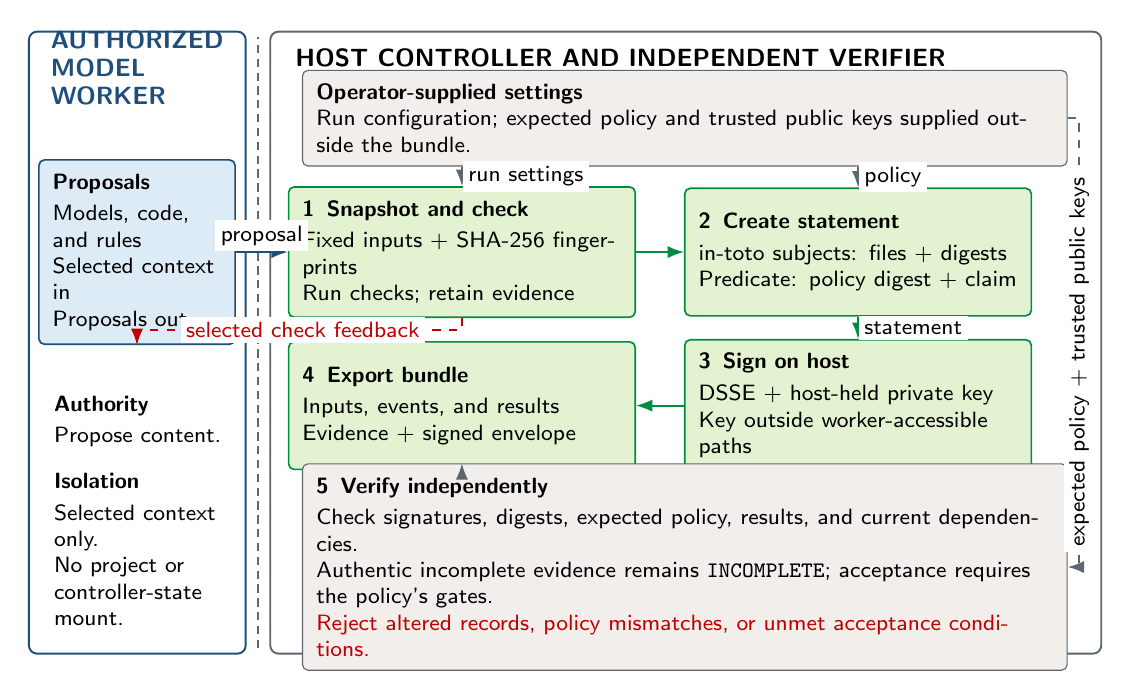
\begin{tikzpicture}[
  x=.78cm,y=1cm,>=Latex,
  font=\sffamily\fontsize{8.2}{9.5}\selectfont,
  stage/.style={draw,rounded corners=2pt,line width=.6pt,align=left,
    inner sep=5pt,text width=4.05cm,minimum height=1.62cm},
  flow/.style={->,line width=.65pt},
  labeltext/.style={font=\sffamily\fontsize{7.6}{8.8}\selectfont,fill=white,inner sep=2pt},
  titletext/.style={font=\sffamily\fontsize{8.6}{10}\selectfont\bfseries,anchor=west}
]
\path[use as bounding box] (0,0) rectangle (17.5,8.0);
\draw[scpBlue,rounded corners=3pt,line width=.7pt] (.02,.05) rectangle (3.55,7.95);
\draw[scpGray,rounded corners=3pt,line width=.7pt] (3.95,.05) rectangle (17.48,7.95);
\draw[scpGray,densely dashed,line width=.6pt] (3.75,.12) -- (3.75,7.88);

\node[titletext,text=scpBlue,align=left,text width=2.28cm] at (.22,7.49) {AUTHORIZED\\MODEL WORKER};
\node[titletext] at (4.2,7.62) {HOST CONTROLLER AND INDEPENDENT VERIFIER};

\node[scpRecord,draw,rounded corners=2pt,align=left,
  text width=9.36cm,inner sep=5pt,minimum height=.9cm] (operator) at (10.7,6.85)
  {\textbf{Operator-supplied settings}\\
   Run configuration; expected policy and trusted public keys supplied outside the bundle.};

\node[stage,scpProposal,text width=2.14cm,minimum height=1.55cm] (worker) at (1.78,5.15)
  {\textbf{Proposals}\\[2pt]
   Models, code, and rules\\
   Selected context in\\
   Proposals out};

\node[stage,scpCheck] (snapshot) at (7.07,5.15)
  {\textbf{1\enspace Snapshot and check}\\[2pt]
   Fixed inputs + SHA-256 fingerprints\\
   Run checks; retain evidence};

\node[stage,scpCheck] (statement) at (13.52,5.15)
  {\textbf{2\enspace Create statement}\\[2pt]
   in-toto subjects: files + digests\\
   Predicate: policy digest + claim};

\node[stage,scpCheck] (sign) at (13.52,3.2)
  {\textbf{3\enspace Sign on host}\\[2pt]
   DSSE + host-held private key\\
   Key outside worker-accessible paths};

\node[stage,scpCheck] (export) at (7.07,3.2)
  {\textbf{4\enspace Export bundle}\\[2pt]
   Inputs, events, and results\\
   Evidence + signed envelope};

\node[draw,scpRecord,rounded corners=2pt,align=left,
  text width=9.36cm,inner sep=5pt,minimum height=1.55cm] (verify) at (10.7,1.15)
  {\textbf{5\enspace Verify independently}\\[2pt]
   Check signatures, digests, expected policy, results, and current dependencies.\\
   Authentic incomplete evidence remains \texttt{INCOMPLETE}; acceptance requires the policy's gates.\\
   \textcolor{scpRed}{Reject altered records, policy mismatches, or unmet acceptance conditions.}};

\draw[flow,scpDataFlow] (worker.east) -- node[labeltext,above]{proposal} (snapshot.west);
\draw[flow,scpCheckFlow] (snapshot.east) -- (statement.west);
\draw[flow,scpCheckFlow] (statement.south) -- node[labeltext,right]{statement} (sign.north);
\draw[flow,scpCheckFlow] (sign.west) -- (export.east);
\draw[flow,scpRecordFlow] (export.south) -- (export.south |- verify.north);
\draw[flow,scpRecordFlow,dashed] (operator.south -| snapshot.north) --
  node[labeltext,right]{run settings} (snapshot.north);
\draw[flow,scpRecordFlow,dashed] (operator.south -| statement.north) --
  node[labeltext,right]{policy} (statement.north);
\draw[flow,scpRecordFlow,dashed] (operator.east) -- (17.12,6.85) -- (17.12,1.15) -- (verify.east);
\node[labeltext,rotate=90] at (17.12,3.75) {expected policy + trusted public keys};

\draw[flow,scpRepairFlow] (snapshot.south) -- (7.07,4.16) -- (1.78,4.16) -- (worker.south);
\node[labeltext,text=scpRed] at (4.48,4.16) {selected check feedback};

\node[align=left,anchor=north west,text width=2.20cm] at (.27,3.45)
  {\textbf{Authority}\\[2pt]
   Propose content.\\[7pt]
   \textbf{Isolation}\\[2pt]
   Selected context only.\\
   No project or controller-state mount.};
\end{tikzpicture}

\caption{Accountability boundary and optional evidence export in \workbench{}~\cite{scpCheckpoint,intotoStatement,dsse}. The worker proposes artifacts; host services record checks and create a signed claim about selected evidence. Steps 1--4 prepare and export that record; step 5 checks it against independently supplied policy and trusted keys. A signature establishes the integrity and origin of the signed record. Local human authorization and acceptance of engineering obligations require their own recorded decisions and checks.}
\Description{A model worker proposes artifacts across an authority boundary. The host snapshots and checks inputs, constructs a statement, signs it, exports a bundle, and independently verifies it using supplied policy and keys.}
\label{fig:attestation}
\end{figure}

\workbench{} governs a target system's models, code, and proofs (Figure~\ref{fig:engineering-stack}). The worker proposes artifacts; host services retain checks and decisions and optionally export signed evidence (Figure~\ref{fig:attestation})~\cite{scpCheckpoint}.

\subsection{Approved Scope and Campaign Records}
At setup, the engineer approves the \emph{scope}: the obligations, assumptions, required checks, and limits for the task. Acceptance requires every mandatory check in that scope to pass on current reviewed contents with matching approval. Authorized exclusions retain their reasons and failed evidence without verification credit.

The algorithms use $\mathcal{C}$ for the \emph{campaign record}: requirements and sources, artifact and rule versions, checks, decisions, scope, and resource consumption. A requirement table links source passages to their interpretation and evidence. Identifiers retrieve these records; fingerprints identify the exact contents checked or approved. Records also name the agent or human responsible for a proposal, check, or decision. Section~\ref{sec:fidelity} follows this review process, and Section~\ref{sec:attestation} explains authorization and signed export.

\subsection{Execution Environments and Shared Records}
\label{sec:execution-environments}
The execution service prepares inputs, invokes tools, and retains results. The engineer delegates generation, checks, and permitted repairs within approved limits on scope, time, tokens, and access to files and context. Changes to requirements, assumptions, or limits require a decision tied to the affected revision. The Python package exposes these services through the browser and command-line interface~\cite{scpCheckpoint}. The measured Workbench snapshot contains 8,255 implementation lines across 51 Python files (Appendix~\ref{app:evaluation-details}).

For example, \texttt{generate\_and\_check}$(t,c)$ in \texttt{development.py} processes task $t$ within campaign $c$, a group of tasks sharing resource limits. It checks approval and input versions, requests a budgeted proposal, prepares its workspace, and runs configured checks. The archive links each result to the task, model call, source inventory, command, and diagnostics. On continuation, the controller checks the current inputs and approval and carries prior charges forward.

Each case and comparison arm starts in a separate workspace. The host assembles the dispatch from declared task files and selected rule versions. An authorized continuation can pass the preceding candidate and diagnostics as inputs to a fresh worker. In the audited SNG runs the worker used an ephemeral Codex session, a temporary worker home, a cleared environment, allowlisted mounts, and selected context supplied through standard input. Tool network access was disabled. Formal checks use separate output directories, and common tool installations and caches can be shared. Runtime scripts build images in containers and launch configured QEMU guests. The host archive retains workspace identities, inputs, commands, outcomes, and observation scopes~\cite{scpCheckpoint,checkpointResults}.

These workspaces and their linked records also supply the experience used for learning. Verbalization turns selected requirements, attempts, diagnostics, and checked results into written lessons that can guide later work within the campaign or on another system (Section~\ref{sec:learning}).

\begin{figure}[t]
\centering
% R18: restored eight-exchange handoff, matching the user-supplied handoff.tex.
% Full-width handoff sequence. Body only; wrap in figure*.
% Requires diagram-style and arrows.meta. Numbered arrows identify events,
% Actor inputs are detailed in the adjacent prose; the header identifies roles.
% Numbered exchanges do not imply successful completion. The single-user CLI/UI share persistent records.
% Neutral panels and black data paths remain legible in print. Dashed red paths
% mark authorization-dependent transitions; wording and numbers also encode meaning.
% The engineer is outside both managed-worker and host-control frames.
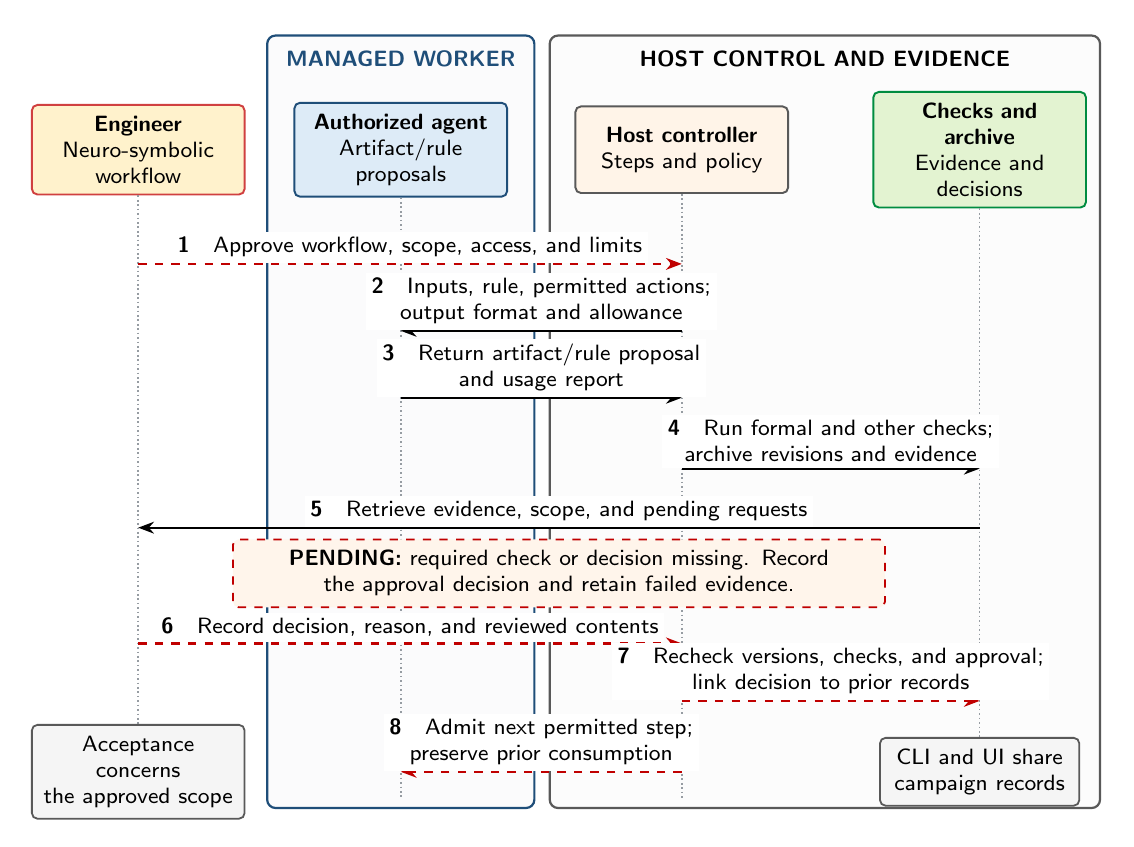
\begin{tikzpicture}[
 x=.78cm,y=1cm,font=\sffamily\fontsize{8.2}{9.4}\selectfont,
 actor/.style={draw=black!65,fill=black!4,text=black,line width=.7pt,rounded corners=2pt,align=center,
   text width=2.42cm,minimum height=1.10cm,inner sep=4pt},
 flow/.style={-{Stealth[length=2.0mm,width=1.5mm]},draw=black,line width=.8pt},
 authorized/.style={draw=scpRed,dashed,line width=.9pt},
 label/.style={align=center,fill=white,inner sep=2pt},
 note/.style={draw=black!65,fill=black!4,text=black,line width=.65pt,rounded corners=2pt,align=center,inner sep=4pt}
]
\path[use as bounding box] (-.3,2.05) rectangle (17.25,-8.00);
\path[draw=scpBlue,fill=scpBlue!2,line width=.8pt,rounded corners=3pt]
 (3.60,1.95) rectangle (7.95,-7.86);
\path[draw=black!65,fill=black!1,line width=.8pt,rounded corners=3pt]
 (8.20,1.95) rectangle (17.16,-7.86);
\node[font=\sffamily\bfseries\fontsize{8.1}{9.3}\selectfont,text=scpBlue]
 at (5.775,1.65) {MANAGED WORKER};
\node[font=\sffamily\bfseries\fontsize{8.1}{9.3}\selectfont]
 at (12.68,1.65) {HOST CONTROL AND EVIDENCE};
\node[actor,draw=scpRed!75,fill=scpYellowFill] (human) at (1.50,.50) {\textbf{Engineer}\\Neuro-symbolic workflow};
\node[actor,draw=scpBlue,fill=scpBlueFill] (worker) at (5.775,.50) {\textbf{Authorized agent}\\Artifact/rule proposals};
\node[actor,fill=orange!9] (controller) at (10.35,.50) {\textbf{Host controller}\\Steps and policy};
\node[actor,draw=scpGreen,fill=scpGreenFill] (archive) at (15.20,.50) {\textbf{Checks and archive}\\Evidence and decisions};
\foreach \n in {human,controller,worker,archive}
  \draw[draw=scpGray!65,densely dotted,line width=.6pt] (\n.south) -- (\n.south |- 0,-7.73);
\draw[flow,authorized] (1.50,-.95) -- node[label,above]{\textbf{1}\quad Approve workflow, scope, access, and limits} (10.35,-.95);
\draw[flow] (10.35,-1.80) -- node[label,above]{\textbf{2}\quad Inputs, rule, permitted actions;\\output format and allowance} (5.775,-1.80);
\draw[flow] (5.775,-2.65) -- node[label,above]{\textbf{3}\quad Return artifact/rule proposal\\and usage report} (10.35,-2.65);
\draw[flow] (10.35,-3.55) -- node[label,above]{\textbf{4}\quad Run formal and other checks;\\archive revisions and evidence} (15.20,-3.55);
\draw[flow] (15.20,-4.30) -- node[label,above]{\textbf{5}\quad Retrieve evidence, scope, and pending requests} (1.50,-4.30);
\node[note,draw=scpRed,fill=orange!8,dashed,text width=8.0cm] at (8.35,-4.88)
  {\textbf{PENDING:} required check or decision missing. Record the approval decision and retain failed evidence.};
\draw[flow,authorized] (1.50,-5.77) -- node[label,above]{\textbf{6}\quad Record decision, reason, and reviewed contents} (10.35,-5.77);
\draw[flow,authorized] (10.35,-6.50) -- node[label,above]{\textbf{7}\quad Recheck versions, checks, and approval;\\link decision to prior records} (15.20,-6.50);
\draw[flow,authorized] (10.35,-7.40) -- node[label,above]{\textbf{8}\quad Admit next permitted step;\\preserve prior consumption} (5.775,-7.40);
\node[note,text width=2.25cm] at (15.20,-7.40) {CLI and UI share\\campaign records};
\node[note,text width=2.42cm] at (1.50,-7.40) {Acceptance concerns\\the approved scope};
\end{tikzpicture}

\caption{Illustrative controlled handoff in \workbench{}~\cite{scpCheckpoint}. The eight numbered exchanges connect approved setup, bounded proposals, host checks, evidence retrieval, and recorded human decisions. The worker and host have separate responsibilities; a review request (5) and the recorded review decision (6) are separate records. Each subsequent task receives the selected rule revision and available allowance (2, 8), while prior outcomes and consumption remain linked to the case. Section~\ref{sec:control-handoff} follows the same numbers.}
\Description{Eight numbered interactions connect operator setup, agent proposals, host checks, evidence recording, review requests, decisions, retrieval, and continuation under remaining allowance.}
\label{fig:control-handoff}
\end{figure}






\section{Scoped Review and Attestation}
\label{sec:attestation}
\label{sec:scoped-attestation}
The campaign record identifies who proposed, checked, and approved a revision. Fingerprints bind those actions to exact contents; authorization checks govern protected actions, and signed exports support independent checking of the evidence.

\subsection{Identify What Was Reviewed}
Adding $L<U$ changes the heater model's fingerprint and requires review of the revised model and its new assumption. A decision covers identified task, rule, artifact, outcome, assumption, and scope records~\cite{scpCheckpoint}. Before a protected action, the controller rechecks the reviewed contents and current approval. A mismatch makes the earlier decision inapplicable to the changed contents and returns the action for review. The history retains the responsible agent or human identifier, the decision, its rationale, and the affected versions. These links establish responsibility during an audit.

\begin{algorithm}[!htbp]
\caption{Review a scope and check an optional signed export}
\label{alg:attestation}
\KwIn{Campaign record $\mathcal{C}$; available human decisions; optional export policy and trusted keys.}
\KwOut{Updated $\mathcal{C}$; local review outcome $q$; export verdict $v$.}
\scpPhase{Record decisions about the current scope}
Refresh evidence and scope; set $q$ to \scpStatus{pending}\nllabel{ln:review-resolve}\;
\ForEach{available decision}{
  \If{a grant or deferral concerns changed contents}{
    Set $q$ to \scpStatus{stale}; stop this loop\;
  }
  \If{acceptance is rejected}{
    Record the rejection; set $q$ to \scpStatus{rejected}; stop this loop\;
  }
  Apply authorized scope changes, deferrals, or revocations; preserve original outcomes\;
  \If{the human decision grants acceptance}{
    Recheck the subject fingerprint and mandatory scoped checks together; approve only if they pass\;
  }
  Refresh the campaign record and the contents under review\;
}
\If{required contents have changed}{Set $q$ to \scpStatus{stale}\;}
\If{$q$ is neither stale nor rejected}{
  Set $q$ to accepted only if every mandatory check in the approved scope passes and its approval is current\nllabel{ln:review-eligible-end}\;
}
\scpPhase{Check a signed export, when requested}
\If{no export is requested}{\Return $q$, \scpStatus{not exported}\nllabel{ln:review-noexport}\;}
Package selected run evidence and sign it on the host\;
Check the signature, contents, and claimed result against the external policy and trusted keys; obtain $v$\;
\Return $q,v$\nllabel{ln:review-return}\;
\end{algorithm}


Local acceptance requires matching reviewed contents and dependencies, passing evidence for every included mandatory check, and current approval of that scope. A human can authorize partial release by recording exclusions and their reasons; deferred obligations remain required. Failed outcomes remain in the history. When the required checks and reviews pass, the task is complete within its approved scope. Algorithm~\ref{alg:attestation} records these decisions and optionally exports a signed claim.

\subsection{Signed Evidence and Independent Checks}
\label{sec:signed-export}
Figure~\ref{fig:attestation} follows five steps. \textbf{1--2. Check and describe.} The host snapshots inputs and records checks. An \emph{in-toto Statement} names files and fingerprints as its \emph{subjects}; its \emph{predicate} states the claim and policy~\cite{intotoStatement}.

\textbf{3--4. Sign and export.} A \emph{Dead Simple Signing Envelope} (DSSE) contains the statement, data-format label, and signatures covering both~\cite{dsse}. The \emph{bundle} contains this envelope and supporting files. The private key remains outside worker-accessible directories.

\textbf{5. Check independently.} The receiver supplies the expected policy and trusted keys. The verifier checks signatures, file inventory and fingerprints, configuration, dependencies, and recorded results. Altered contents or inconsistent claims are rejected. Authentic evidence from unfinished work can yield \texttt{INCOMPLETE}; \texttt{ACCEPTED} also requires the recorded engineering-acceptance flag and passing evidence for the verifier's required engineering checks~\cite{scpCheckpoint}. The signed record preserves the identity of the exported evidence, while the local review records preserve approval and responsibility for the declared scope.

\section{Budgeted Supervised Meta-Learning}
\label{sec:learning}

The handoff in Figure~\ref{fig:control-handoff} supplies reviewed tasks with selected guidance. The learning process in Figure~\ref{fig:handoff} uses attempts and checks from campaign workspaces to revise that guidance. It repeats within a campaign and carries accumulated lessons into later systems. The heater case shows how a failure can motivate a new rule and define where it applies.

\begin{figure}[t]
\centering
% Supervised rule-evolution overview. Layers group existing records;
% they are not new wiki folders, immutable storage, or qualified skills.
% Stage numbers match handoff.tex; Algorithm 2 gives the detailed procedure.
\begingroup
\hyphenpenalty=10000
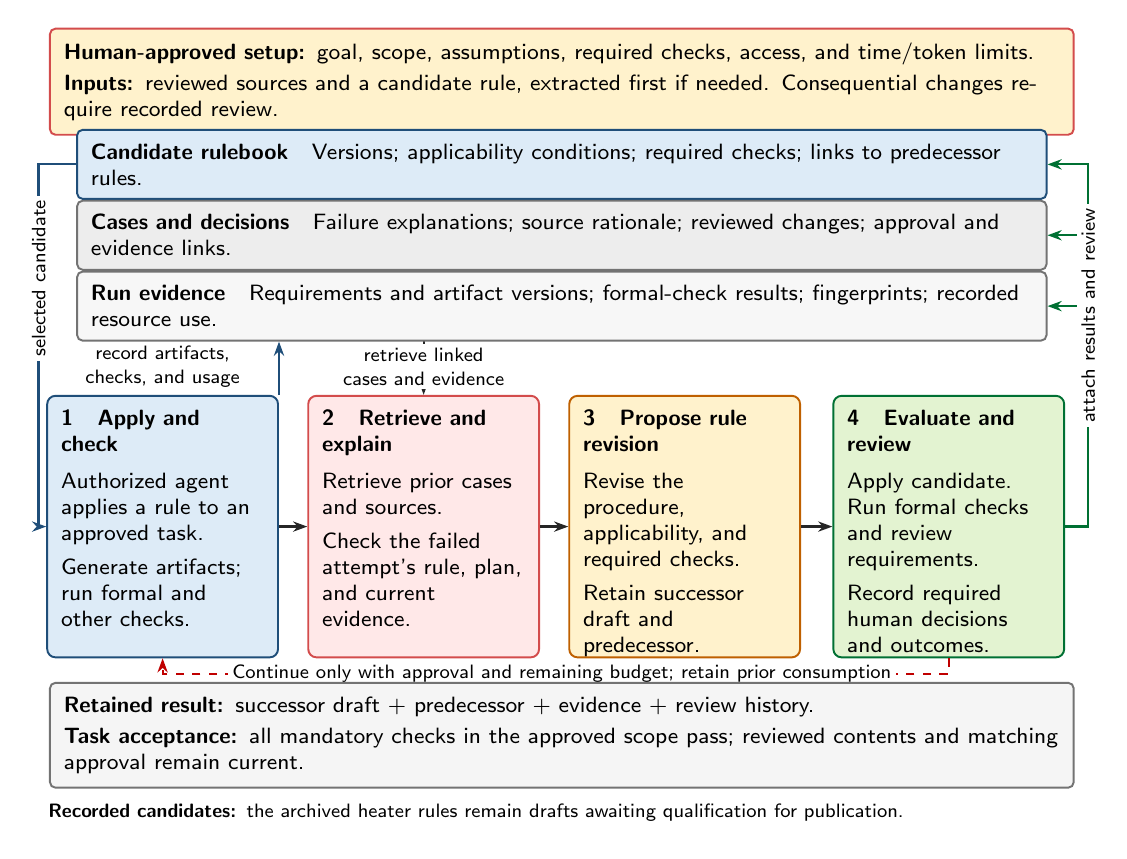
\begin{tikzpicture}[
 x=.78cm,y=1cm,font=\sffamily\fontsize{8}{9.4}\selectfont,
 band/.style={draw=black!55,fill=black!4,line width=.7pt,rounded corners=2pt,
   text=black,align=left,text width=11.96cm,minimum height=.64cm,inner sep=5pt},
 evoStep/.style={draw=black!60,line width=.7pt,rounded corners=3pt,text=black,
   align=left,text width=2.58cm,minimum height=3.30cm,inner sep=5pt},
 flow/.style={-{Stealth[length=1.8mm,width=1.3mm]},draw=black!85,line width=.8pt},
 label/.style={font=\sffamily\fontsize{7.3}{8.5}\selectfont,
   fill=white,align=center,inner sep=1.5pt},
 note/.style={font=\sffamily\fontsize{7.3}{8.5}\selectfont,align=left}
]
\node[band,text width=12.65cm,minimum height=.91cm,fill=scpYellowFill,draw=scpRed!70]
 (setup) at (8.7,8.40) {\textbf{Human-approved setup:} goal, scope, assumptions, required checks, access, and time/token limits.\\[2pt]
 \textbf{Inputs:} reviewed sources and a candidate rule, extracted first if needed. Consequential changes require recorded review.};
\node[band,fill=scpBlueFill,draw=scpBlue] (rules) at (8.7,7.35)
 {\textbf{Candidate rulebook}\quad Versions; applicability conditions; required checks; links to predecessor rules.};
\node[band,fill=black!7] (cases) at (8.7,6.45)
 {\textbf{Cases and decisions}\quad Failure explanations; source rationale; reviewed changes; approval and evidence links.};
\node[band,fill=black!3] (evidence) at (8.7,5.55)
 {\textbf{Run evidence}\quad Requirements and artifact versions; formal-check results; fingerprints; recorded resource use.};
\node[evoStep,draw=scpBlue,fill=scpBlueFill] (run) at (2.20,2.75)
 {\parbox[t][2.97cm][t]{2.58cm}{\raggedright\textbf{1\quad Apply and check}\\[4pt]
 Authorized agent applies a rule to an approved task.\\[3pt]
 Generate artifacts; run formal and other checks.}};
\node[evoStep,draw=scpRed!70,fill=scpRedFill] (diagnose) at (6.45,2.75)
 {\parbox[t][2.97cm][t]{2.58cm}{\raggedright\textbf{2\quad Retrieve and explain}\\[4pt]
 Retrieve prior cases and sources.\\[3pt]
 Check the failed attempt's rule, plan, and current evidence.}};
\node[evoStep,draw=orange!75!black,fill=scpYellowFill] (revise) at (10.70,2.75)
 {\parbox[t][2.97cm][t]{2.58cm}{\raggedright\textbf{3\quad Propose rule revision}\\[4pt]
 Revise the procedure, applicability, and required checks.\\[3pt]
 Retain successor draft and predecessor.}};
\node[evoStep,draw=scpGreen!80!black,fill=scpGreenFill] (assess) at (15.00,2.75)
 {\parbox[t][2.97cm][t]{2.58cm}{\raggedright\textbf{4\quad Evaluate and review}\\[4pt]
 Apply candidate. Run formal checks and review requirements.\\[3pt]
 Record required human decisions and outcomes.}};
% Record-layer connections are distinct from the ordered processing steps.
\draw[flow,draw=scpBlue] (rules.west) -- (.18,7.35) -- (.18,2.75) -- (run.west);
\node[label,rotate=90] at (.18,5.90) {selected candidate};
\draw[flow,draw=scpBlue] (run.north east) -- (evidence.south -| run.north east);
\node[label] at (2.20,4.78) {record artifacts,\\checks, and usage};
\begin{scope}[on background layer]
 \draw[flow] (cases.south -| diagnose.north) -- (diagnose.north);
\end{scope}
\node[label] at (6.45,4.78) {retrieve linked\\cases and evidence};
\draw[flow,draw=scpGreen!80!black] (assess.east) -- (17.27,2.75) -- (17.27,7.35) -- (rules.east);
\draw[flow,draw=scpGreen!80!black] (17.27,6.45) -- (cases.east);
\draw[flow,draw=scpGreen!80!black] (17.27,5.55) -- (evidence.east);
\node[label,rotate=90] at (17.27,5.43) {attach results and review};
\draw[flow] (run.east) -- (diagnose.west);
\draw[flow] (diagnose.east) -- (revise.west);
\draw[flow] (revise.east) -- (assess.west);
\draw[flow,draw=scpRed,dashed] (assess.south) -- (15.00,.88) -- (2.20,.88) -- (run.south);
\node[label] at (8.7,.88) {Continue only with approval and remaining budget; retain prior consumption};
\node[band,text width=12.65cm,minimum height=1.0cm,fill=black!4] at (8.7,.10)
 {\textbf{Retained result:} successor draft + predecessor + evidence + review history.\\[2pt]
 \textbf{Task acceptance:} all mandatory checks in the approved scope pass; reviewed contents and matching approval remain current.};
\node[note,text width=13.2cm,anchor=north west] at (.18,-.65)
 {\textbf{Recorded candidates:} the archived heater rules remain drafts awaiting qualification for publication.};
\end{tikzpicture}
\endgroup

\caption{Supervised rule evolution in \workbench{}. A layered presentation inspired by WikiSkill~\cite{tang2026wikiskill} separates recorded evidence, cases and decisions, and candidate guidance. The four stages apply a candidate, interpret prior experience, propose a revision, and evaluate it under review. Updates retain the preceding rule and supporting records. Further attempts require current approval and remaining allowance. Acceptance concerns the reviewed task scope; candidate rules require independent tests before publication for reuse. Section~\ref{sec:handoff} explains the stages; Figure~\ref{fig:evolution} gives a concrete rule history.}
\Description{Three persistent layers store evidence, reviewed cases, and candidate guidance. Four stages apply guidance, interpret experience, propose revised rules, and run formal checks and review within approved scope.}
\label{fig:handoff}
\end{figure}

\subsection{Controlled Handoff}
\label{sec:control-handoff}
A \emph{handoff} supplies an authorized agent with inputs and permitted actions and returns its proposal for host checks. Figure~\ref{fig:control-handoff} follows eight exchanges.

\textbf{1--2. Approve and prepare.} The engineer approves the workflow, scope, access, and limits (1). The harness retrieves current inputs and the selected rule, checks allowance, and specifies permitted actions and output format (2). Evaluator-only artifacts remain separate from dispatched context. Shared task documents and approved reference-derived supplements are declared inputs whose provenance is retained.

\textbf{3--4. Propose and check.} The worker returns an artifact or rule proposal and usage report (3). The host runs formal and other checks and records versions, outcomes, and fingerprints (4).

\textbf{5--7. Retrieve and review.} The engineer retrieves pending requests and evidence (5), records the decision and rationale (6), and the host checks its contents and links it to prior records (7). A request alone grants no authority.

\textbf{8. Continue within limits.} Agents select permitted repairs while approval and allowance remain current. Expanding scope, assumptions, access, or budgets requires renewed human authorization. Prior charges and unresolved outcomes remain recorded~\cite{scpCheckpoint}.

A revised rule selected for another task enters at exchange~2; its outcomes return at exchange~4. Figure~\ref{fig:handoff} explains how this experience informs revision.

\begin{figure}[t]
\centering
% Condensed from public draft-rules.json, GOLDEN-DEFECT-CURATION-001.
% Selected actual revisions draft-1, draft-2, draft-4; draft-3 is omitted.
% Approval of the case premise is distinct from qualification of any rule.
% The input is a documented SMT diagnosis for a contract fragment, not a
% recovered full-system GUMBOX execution trace.
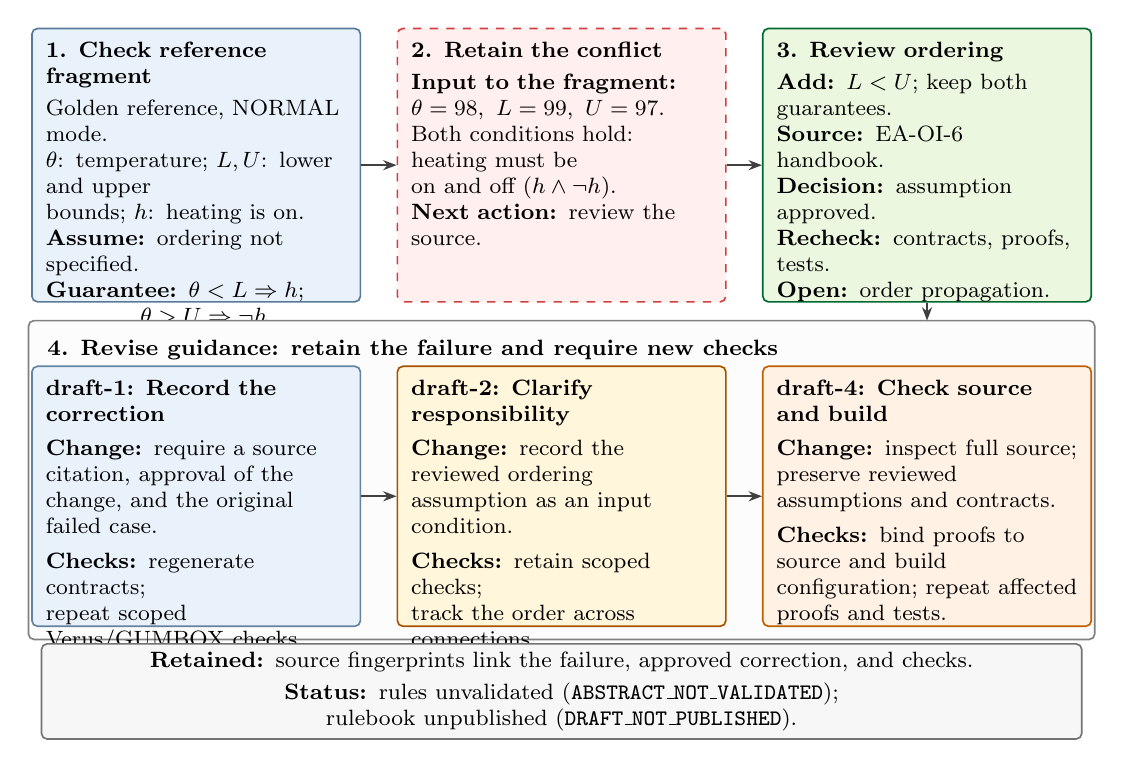
\begin{tikzpicture}[
 x=.78cm,y=1cm,
 font=\fontsize{8}{9.4}\selectfont,
 card/.style={draw=black!65,text=black,rounded corners=2pt,line width=.6pt,
   align=left,inner sep=5pt},
 record/.style={card,text width=3.82cm,minimum height=3.47cm,anchor=north},
 candidate/.style={card,text width=3.82cm,minimum height=3.30cm,anchor=north},
 arrow/.style={-{Stealth[length=1.7mm]},draw=black!75,line width=.7pt}
]
\node[record,draw=scpBlue!75,fill=scpBlueFill!65!white] (requirements) at (2.7,7.25)
 {\begin{minipage}[t][3.12cm][t]{3.82cm}\raggedright\textbf{1. Check reference fragment}\\[2pt]
  Golden reference, NORMAL mode.\\
  $\theta$: temperature; $L,U$: lower and upper\\
  bounds; $h$: heating is on.\\
  \textbf{Assume:} ordering not specified.\\
  \textbf{Guarantee:} $\theta<L\Rightarrow h$;\\
  \hspace*{1.20cm}$\theta>U\Rightarrow\neg h$.\end{minipage}};
\node[record,draw=scpRed!75,fill=scpRedFill!70!white,dashed] (conflict) at (8.65,7.25)
 {\begin{minipage}[t][3.12cm][t]{3.82cm}\raggedright\textbf{2. Retain the conflict}\\[2pt]
  \textbf{Input to the fragment:}\\
  $\theta=98,\ L=99,\ U=97$.\\
  Both conditions hold: heating must be\\
  on and off ($h\land\neg h$).\\
  \textbf{Next action:} review the source.\end{minipage}};
\node[record,draw=scpGreen!75!black,fill=scpGreenFill!70!white] (decision) at (14.6,7.25)
 {\begin{minipage}[t][3.12cm][t]{3.82cm}\raggedright\textbf{3. Review ordering}\\[2pt]
  \textbf{Add:} $L<U$; keep both guarantees.\\
  \textbf{Source:} EA-OI-6 handbook.\\
  \textbf{Decision:} assumption approved.\\
  \textbf{Recheck:} contracts, proofs, tests.\\
  \textbf{Open:} order propagation.\end{minipage}};
\draw[arrow] (requirements.east) -- (conflict.west);
\draw[arrow] (conflict.east) -- (decision.west);
\path[draw=black!50,fill=black!1,rounded corners=2pt,line width=.6pt]
 (-.03,-.52) rectangle (17.33,3.53);
\node[anchor=north west,font=\fontsize{8.2}{9.5}\selectfont\bfseries] at (.12,3.41)
 {4. Revise guidance: retain the failure and require new checks};
\node[candidate,draw=scpBlue!70,fill=scpBlueFill!65!white] (first) at (2.7,2.96)
 {\begin{minipage}[t][2.95cm][t]{3.82cm}\raggedright\textbf{draft-1: Record the correction}\\[3pt]
  \textbf{Change:} require a source citation, approval of the change, and the original failed case.\\[3pt]
  \textbf{Checks:} regenerate contracts;\\
  repeat scoped Verus/GUMBOX checks.\end{minipage}};
\node[candidate,draw=orange!65!black,fill=scpYellowFill!70!white] (second) at (8.65,2.96)
 {\begin{minipage}[t][2.95cm][t]{3.82cm}\raggedright\textbf{draft-2: Clarify responsibility}\\[3pt]
  \textbf{Change:} record the reviewed ordering assumption as an input condition.\\[3pt]
  \textbf{Checks:} retain scoped checks;\\
  track the order across connections.\end{minipage}};
\node[candidate,draw=orange!75!black,fill=orange!10] (third) at (14.6,2.96)
 {\begin{minipage}[t][2.95cm][t]{3.82cm}\raggedright\textbf{draft-4: Check source and build}\\[3pt]
  \textbf{Change:} inspect full source; preserve reviewed assumptions and contracts.\\[3pt]
  \textbf{Checks:} bind proofs to source and build configuration; repeat affected proofs and tests.\end{minipage}};
% Fixed-height cards keep both revision arrows horizontal.
\draw[arrow] (first.east) -- (second.west);
\draw[arrow] (second.east) -- (third.west);
\draw[arrow] (decision.south) -- (14.6,3.53);
\node[card,draw=black!55,fill=black!3,text width=13.0cm,align=center,minimum height=.93cm,inner sep=3pt] at (8.65,-1.18)
 {\textbf{Retained:} source fingerprints link the failure, approved correction, and checks.\\[2pt]
  \textbf{Status:} rules unvalidated (\texttt{ABSTRACT\_NOT\_VALIDATED}); rulebook unpublished (\texttt{DRAFT\_NOT\_PUBLISHED}).};
\end{tikzpicture}

\caption{A heater reference case becomes a source of candidate guidance~\cite{scpCheckpoint}. Steps 1--2 expose conflicting guarantees in the contract fragment. Step 3 records review of an added ordering assumption and the checks required afterwards. Step 4 shows selected rule revisions with links to sources and checks; drafts 1, 2, and 4 are selected from the archive. The added assumption was approved, while the candidate rules await qualification. Horizontal arrows show revision order; intermediate and later drafts are omitted.}
\Description{A temperature contract permits conflicting heater commands without an ordering assumption. Review adds an assumption and records supporting evidence. Three selected draft rules retain that lesson and remain pending independent qualification.}
\label{fig:evolution}
\end{figure}

\subsection{Supervised Rule Evolution}
\label{sec:handoff}
Figure~\ref{fig:handoff} connects run evidence, cases and decisions, and candidate rules through four stages governed by the handoff.

\textbf{1. Apply and check.} Extract an initial candidate from reviewed sources when needed. Apply the selected rule to an approved task, run formal and other checks, and retain versions, outcomes, and resource use.

\textbf{2. Retrieve and explain.} Retrieve the attempt, source context, and review history. Express the reusable structure, procedure, or concept suggested by that experience. Refining a rule requires current failed evidence from that candidate and its approved plan.

\textbf{3. Propose a revision.} State the revised procedure, the tasks it applies to, and the checks it requires. Retain the preceding rule and supporting evidence.

\textbf{4. Evaluate and review.} Apply the candidate with fresh checks and requirements review. Record consequential decisions separately. Acceptance concerns the approved task scope; publishing a reusable rule requires independent qualification.

Missing evidence, approval, or allowance leaves work pending. Continuation retains earlier consumption and remains part of the same workflow. Approved exclusions retain failed outcomes without verification credit~\cite{scpCheckpoint}.




\subsection{From Experience to a Candidate Rule}
Learning turns recorded attempts, diagnostics, and checks into reusable guidance. A \emph{meta-rule} states when it applies, its assumptions, a procedure, and the required checks. The \emph{Generalizer} extracts a procedure shared by related tasks; the \emph{Specializer} supplies the current interfaces, assumptions, and obligations. These strategies use the same model worker. Each proposed rule retains its sources and earlier versions, extending SCP's supervised learning and repair process with persistent review and accounting~\cite{tahat2026scp,scpCheckpoint}.

The file handoff in Section~\ref{sec:execution-environments} makes the reusable knowledge explicit. A new target receives a rule snapshot with its own task inputs. The host archive retains the diagnostic, rule revision, and check that motivated each lesson, so a subsequent attempt can refine the rule and leave the earlier history inspectable. Section~\ref{sec:evaluation} identifies the rules carried between the evaluated cases.

Earlier SCP used a similarity comparison when considering formalizations~\cite{tahat2026scp}. The workbench computes cosine distance to retrieve related rules and to compare contract features after architecture checking. It also records model forecasts with explanations. These signals can help prioritize interpretation and review (Section~\ref{sec:fidelity}).

An early \emph{semantic gate} would use the predicted agreement between English requirements and a proposed interpretation to choose whether to proceed to formalization, refine the interpretation, or request review. Automatic admission and branch ranking are proposed extensions of the available comparison and forecast services. Formal checks and human review then assess the candidate. Appendix~\ref{app:semantic-budget} gives the representations, cosine geometry, and connection to budgeted candidate selection~\cite{foster2026rpm,tahat2026dascslides}.

\subsection{Learning from the Heater Case}
Figure~\ref{fig:evolution} follows a reference correction (upper row) and the candidate guidance derived from it (lower row).

\textbf{(1) Check the reference contract.} Using the notation of Section~\ref{sec:background}, the heater fragment requires $\theta<L\Rightarrow h$ and $\theta>U\Rightarrow\neg h$ in NORMAL mode, without ordering $L$ and $U$.

\textbf{(2) Retain the conflicting input.} The diagnostic script uses $\theta=98$, $L=99$, and $U=97$: both conditions hold, requiring heating on and off simultaneously~\cite{scpCheckpoint}. This exposes the missing constraint in the fragment; $U=97$ lies outside the handbook's full upper-bound range~\cite{lempia2009faa}. Giving one output priority changes a guarantee; filtering tests changes coverage; adding an ordering assumption restricts inputs. Each repair therefore needs an explanation of how it meets the requirement.

\textbf{(3) Review the assumption.} The repair record approves $L<U$ and retains both guarantees. It cites \texttt{EA-OI-6}, the operator-interface environmental assumption in Lempia and Miller's handbook requiring $L\leq U-1^{\circ}\mathrm{F}$~\cite[Appendix A.3.4, p.~A-11]{lempia2009faa}. Strict ordering gives this margin for integer degree settings; other representations require the margin to be stated explicitly. Review records responsibility for the chosen premise; proof and tests assess the repaired artifact, with internal propagation retained as an obligation.

\textbf{(4) Revise the rule.} The figure shows revisions of \texttt{GOLDEN-\allowbreak{}DEFECT-\allowbreak{}CURATION-001}. \texttt{draft-1} requires cited correction, consent, failure retention, regeneration, and checks with Verus and GumboX. \texttt{draft-2} distinguishes environmental assumptions from software guarantees. \texttt{draft-4} adds the complete sources and build context and requires reassessment of regenerated contracts and proofs. Each revision retains its predecessor and supporting evidence; these archived candidates await qualification for publication~\cite{scpCheckpoint}.

Section~\ref{sec:retrieval} explains retrieval of these linked records.

\subsection{Learning Within an Allowance}
Algorithm~\ref{alg:learning} receives the case, reviewed sources, and an optional candidate selected directly or through the retrieval comparison. It can also extract a new draft from the sources. Algorithm~\ref{alg:requirements-fidelity} supplies the development and fidelity-review procedure.
\noindent\emph{Reading the procedures.}
A \emph{budgeted model step} reserves an allowance, calls the model, records usage, and retains the outcome. It returns \textsc{pending} if another check, decision, allowance, or human instruction is needed. A changed input produces \textsc{stale}, which requires renewed review. Every return keeps the campaign history. Section~\ref{sec:evaluation} reports a failure in retaining a detailed call record; the procedures describe the intended order of operations.

\begin{algorithm}[!htbp]
\caption{Learn a candidate rule from retained campaign experience}
\label{alg:learning}
\KwIn{Campaign record $\mathcal{C}$; reviewed sources $M$; optional draft rule $r$.}
\KwOut{Updated $\mathcal{C}$ and $r$; current task outcome $q$.}
\scpPhase{Prepare the rule}
\If{the source or plan is unapproved}{
  \Return \scpStatus{pending} for review\nllabel{ln:learn-review}\;
}
\If{the reviewed source or plan changed}{
  \Return \scpStatus{stale}\;
}
\If{no draft $r$ is supplied}{
  Extract $r$ from $M$ with a budgeted call\;
  \If{no draft is returned}{\Return \scpStatus{pending}\;}
  Retain $r$, its sources, and the call record\nllabel{ln:learn-extract-end}\;
}
\scpPhase{Apply and revise the rule}
\While{recorded permission and budget permit another attempt}{
  Select a currently approved prepared task $T$\nllabel{ln:learn-task}\;
  \If{no such task is available}{\Return \scpStatus{pending}\;}
  Apply $r$ to $T$ in a budgeted call; check; set $q$\;
  \If{$q$ is not \texttt{NOT\_VALIDATED}}{\Return $q$\;}
  \If{the failure uses another rule or plan}{\Return \scpStatus{rejected}\;}
  \If{diagnostic inputs changed}{\Return \scpStatus{stale}\;}
  Revise $r$ from permitted feedback in a budgeted call\;
  \If{no revision is returned}{\Return \scpStatus{pending}\;}
  Retain both rules, failure, and attempts; use the new rule as $r$\nllabel{ln:learn-successor}\;
}
\Return \scpStatus{pending} for more allowance or human guidance\;
\end{algorithm}


The first phase extracts a draft and retains its origin (lines~\ref{ln:learn-review}--\ref{ln:learn-extract-end}). The second applies it to a reviewed task. Rewriting requires current failed evidence from the same rule and plan, recorded as \texttt{NOT\_VALIDATED}; the revised rule keeps links to the failure and earlier rule (lines~\ref{ln:learn-task}--\ref{ln:learn-successor}).

\paragraph{Resource accounting}
\label{sec:resource-accounting}
The campaign's resource ledger retains time, tokens, and attempts across retries. Process deadlines bound execution; token reservations estimate usage, then the ledger records measured consumption and any excess. The estimate may be lower than the usage reported by the provider. Exhausted allowances or unresolved usage stop calls. Approved extensions preserve prior consumption (Section~\ref{sec:interface}).

\paragraph{Qualification for reuse}
Algorithm~\ref{alg:learning} returns a task outcome and a revised candidate. Publishing that rule uses the separate qualification and approval service, which checks evidence for declared examples. The archived heater drafts retain their qualification status~\cite{scpCheckpoint}.

\section{Requirements Fidelity and Persistent Review}
\label{sec:fidelity}
\label{sec:requirements-workflow}

\emph{Requirements fidelity} means that the checked obligations preserve the reviewed engineering intent. Appendix~\ref{app:requirements-review} illustrates the review and refinement loop. The reviewer reads the English source line by line and builds a requirement table: each obligation has a source passage, an interpretation, its intended model or code representation, and the assumptions needed to check it. Ambiguities, omissions, and proposed changes remain visible for review. This review includes checking extracted text against its source before approving the input.

\subsection{From English Requirements to Checked Evidence}
Semantic assessment examines whether the interpretation and formalization express the requirement. For the heater, the reviewer must decide whether the premise $L<U$ represents the intended environment. Model explanations and comparisons can help identify questions for review. Contract-feature similarity helps locate related obligations; logical equivalence requires an appropriate logical check~\cite{bayless2025arc,tahat2026scp}. Our adaptation of CLOVER connects English requirements, semantic assessment, and verification evidence around the formalization~\cite{sun2024clover}. The proposed predictor would estimate agreement with reviewed intent and the time and tokens for the next attempt. It would use prior reviews and comparable check records to prioritize candidates under the remaining allowance (Appendix~\ref{app:semantic-budget}).

The reviewed task specifies inputs, rule revisions, required checks, and limits. A budgeted proposal proceeds through HAMR generation and the configured checks. Parsing checks syntax and types; architecture comparison checks components and connections; proofs establish contracts under their premises. Tests and runtime observations cover their configured cases and periods. The requirement table connects these results to the original obligations and records unresolved questions. Repairs within approved scope continue the same trajectory with its earlier consumption. Changes to requirements, assumptions, scope, or limits return to human review.

\subsection{Close the Loop with an Identified Decision}
Each campaign record retains its English inputs, candidate revisions, checks, costs, and decisions. Requirement tables and case audits connect the reviewed intent to model contracts and evidence. Fingerprints identify the exact contents covered by a review. Rechecking detects changed contents and triggers reassessment of the affected claims. Each assessment or decision identifies the responsible agent or human reviewer.

A task is complete when every required check and review in its declared scope has passed. The human owner decides release. An approved partial release states the included scope, exclusions, assumptions, and remaining obligations; excluded obligations receive no verification credit. The acceptance conditions in Section~\ref{sec:attestation} bind the decision to current contents and evidence.

The case studies illustrate this process. Isolette source review recovered omitted environmental dependencies and identified timeout and timing discrepancies. Producer/Consumer and SNG audits connected source requirements to model contracts and proof evidence. These reviews establish which interpretations and assumptions the evidence supports. Appendix~\ref{app:requirements-review} gives Algorithm~\ref{alg:requirements-fidelity}; Appendix~\ref{app:coverage-details} follows one SNG requirement through its contracts, proofs, and assumptions.


\section{Evaluation}
\label{sec:evaluation}
\suppressfloats[t]

We evaluate guidance reuse and reconstruction (RQ1), control of repairs and continuation (RQ2), and the connection between reviewed requirements and checked artifacts (RQ3). The cases follow guidance from Isolette Monitor to the Regulator holdout, then examine new construction and later reconstruction for Producer/Consumer and the Simple Network Guard (SNG). We distinguish model checkpoints, successful builds, and bounded runtime observations.

\paragraph{Protocol and timing}
Candidate workspaces isolate runs of the INSPECTA tools~\cite{hardin2025dasc}. Experiment calls requested \texttt{gpt-6-astra} through Codex~0.155.1. In each later reconstruction pair, $K$ receives the common requirements, libraries, and guides, including the shared design supplement where applicable. $K^{+}$ adds a selected rule bundle. Each arm has a 500,000-token allowance and a 24-minute model-stage limit. Each pair reports one trajectory per arm. Completion requires all five specified model checks. Table~\ref{tab:sng-comparison} reports the measured work through that endpoint or the observed stop~\cite{sigplanEmpirical2018}. Appendix~\ref{app:resource-details} gives the configuration, clock definitions, and estimated debits.

\begin{table}[!htbp]
\caption{Later common-input model pairs. Times are in seconds. Dispatch includes client and controller call handling, checks sum the recorded tool intervals, and elapsed time includes gaps. A dash marks an unavailable elapsed interval at that endpoint.}
\label{tab:sng-comparison}
\centering\small
\setlength{\tabcolsep}{4pt}
\begin{tabular}{@{}>{\raggedright\arraybackslash}p{.24\linewidth}>{\raggedright\arraybackslash}p{.24\linewidth}rrrr@{}}
\toprule
Case and arm & Outcome & \shortstack[r]{Measured\\tokens} & Dispatch & Checks & Elapsed \\
\midrule
Producer/Consumer $K$ & HTTP 429 & 48,236 & 36.35 & 17.40 & 57.86 \\
Producer/Consumer $K^{+}$ & Five checks passed & 179,515 & 109.53 & 94.45 & 210.19 \\
SNG $K$ & Repair limit & 388,726 & 682.71 & 362.30 & 1,052.77 \\
SNG $K^{+}$ & Five checks passed & 346,224 & 532.43 & 154.10 & --- \\
\bottomrule
\end{tabular}
\end{table}

\subsection{Isolette: Monitor Guidance and Regulator Continuation}
Isolette regulates an infant incubator~\cite{hatcliff2024isolette}. Monitor supplied training examples and Regulator served as a component holdout for model generation and extension to Rust/Verus. Six successive candidates used draft guidance from preceding attempts. The fifth first passed parsing and architecture capture. Revised, approved English and reference abstractions then supported structural agreement~\cite{isoletteConsolidatedReport2026}.

The revised generation completion was recorded 22\,min 27\,s after revised-input approval. The historical ledger attributes 341,178 measured tokens and 32.43 minutes of summed reservation-to-usage intervals to generation attempts and English preparation, with a separate 1M estimated timeout debit. The repaired Rust continuation completed 11 of 11 component proof/test pairs with 62 conditional obligations. Twenty-nine GumboX and 23 other test functions passed. A Microkit build passed, followed by a 20.008-second observation command including startup. The results cover the approved environmental premises and physical-operator exclusion. Appendix~\ref{app:evaluation-details} gives the review chronology and separately scoped probes.

\subsection{Producer/Consumer: First Construction and Later Reconstruction}
\label{sec:reuse-evaluation}
\paragraph{First construction}
Producer/\allowbreak{}Consumer was held out of the documented Monitor training split~\cite{scpCheckpoint}. The campaign team reports that the first separate workspace received English requirements and existing rulebooks. The worker constructed the SysML v2/GUMBO target from scratch. Its repairs became a source of guidance for later Producer/\allowbreak{}Consumer and SNG work~\cite{producerConsumerConsolidatedReport2026}. A separate historical checkpoint reports 2 of 2 component pairs, 5 of 5 GumboX tests, and 4 of 4 other tests passing on 23 September, with bounded observation. The case-level summary leaves the checked candidate's identity unspecified~\cite{checkpointResults}.

\paragraph{Later paired reconstruction}
The producer's output range $[0,90]$ implies the consumer's assumption $[0,100]$. Both arms received identical English, 15 libraries, nine workflow guides, and the same controller. $K^{+}$ ran first with six general entries from Isolette/HAMR and three from earlier Producer/\allowbreak{}Consumer repairs covering port refinement, effective processor binding, and signed-32 literals.

The five checks cover parsing and types, JVM generation, the Logika connection implication, architecture capture, and effective binding. $K^{+}$ passed the checkpoint and a separate directed-graph comparison. The paired $K$ stopped on HTTP~429, as did a separate authorized follow-up. The paired row describes work observed before interruption, and $K$'s completion time and token use remain unknown. Appendix~\ref{app:resource-details} reports the follow-up timing and the separate 1M estimated debit for each interruption~\cite{producerConsumerConsolidatedReport2026}.

\subsection{SNG: First Construction and Later Reconstruction}
\label{sec:sng-evaluation}
SNG passes classified messages through a gate and filter to a receiver, with contracts for dropping, forwarding, and payload bounds~\cite{hamrTutorials2026}.

\paragraph{First construction with earlier-system rules}
All 11 retained entries at the first guided dispatch came from general rules and earlier system work, including Producer/\allowbreak{}Consumer repairs. Both arms received SNG English and guides with SNG examples. The guided arm also received approved reference-derived design choices. It passed its in-loop model checkpoint with two verified connection units after five repairs and 397,520 measured tokens. The ordinary-input arm stopped after six repairs and 387,144 measured tokens. The differing design inputs limit attribution to guidance (Appendix~\ref{app:evaluation-details}).

\paragraph{Later reconstruction with shared design inputs}
The earlier SNG attempts and recoveries yielded 11 draft SNG lessons. A separate reconstruction supplied $K^{+}$ with 66 selected entries, including those drafts and earlier-system guidance. Both arms used the same English, libraries, guides, approved design supplement, checks, and allowance. The five checks cover parsing and types, Microkit generation, JVM generation, Logika integration, and architecture capture. The guided arm passed all five and a separate directed-graph comparison. It reached the checkpoint with 42,502 fewer measured tokens than $K$ used at its repair-limit stop. Dispatch plus check intervals summed to 686.53\,s for $K^{+}$ at the checkpoint and 1,045.02\,s for $K$ at the stop. The endpoints differ, and the $K$ stop leaves time to completion unknown. This pair evaluates the full supplied bundle (RQ1).

With the five-check checkpoint as the target, $K^{+}$ completed 1/1 at 346,224 measured tokens per completion. $K$ completed 0/1 under the same 500,000-token ceiling. Appendix~\ref{app:resource-details} uses $+\infty$ to display zero completed targets and retains the measured tokens at the stop.

One retained lesson came from a parser rejection. An earlier SysML model used rendered Slang literal syntax. The draft rule distinguishes SysML's \texttt{0 [s32]} from the generated Slang notation. The archive links the rejected attempt to the lesson and matches its text in the supplied 66-entry snapshot (Appendix~\ref{app:evaluation-details}).

\paragraph{Continuation of the later candidate}
A source-preservation check rejected a proposal to remove an existing test function. The controller retained its 78,469-token charge, bringing usage to 424,693. Authorized paid repairs added 151,909 tokens. Two later authorized repairs addressed serialization and initialization without additional experiment-model calls. The guided trajectory used 576,602 worker tokens and 18.72 minutes of dispatch across eight calls. From guided controller start to observation end it took 2\,h 31\,min 21\,s, including approval pauses. The $K$ arm's dependent checks were \texttt{NOT\_RUN}. Table~\ref{tab:sng-completion} reports the guided build and checks.

\begin{table}[!htbp]
\caption{Artifact provenance and evidence for the later SNG $K^{+}$ trajectory~\cite{sngFinalReport2026}.}
\label{tab:sng-completion}
\centering\small
\begin{tabular}{@{}>{\raggedright\arraybackslash}p{.16\linewidth}>{\raggedright\arraybackslash}p{.32\linewidth}>{\raggedright\arraybackslash}p{.47\linewidth}@{}}
\toprule
Stage & Produced artifact & Check or observation \\
\midrule
Model & SysML v2/GUMBO from the declared English, guides, and design inputs. & Five model checks and directed-graph comparison passed. \\
Code and proofs & HAMR-generated infrastructure and contracts with repaired Rust and Slang application artifacts. & Verus verified 32 target-crate units, including six initialization/composition checks. Six English component relations were checked under recorded premises. \\
Tests & Rust and Slang/JVM test results. & 33 Rust test functions and 808 JVM test cases passed. \\
Image & 4,957,232-byte Microkit loader image. & Verification-enabled build passed in 103.501\,s. Build and observation inventories matched 201 paths. \\
Runtime & QEMU loader run and receiver log. & 20.033\,s after readiness, 18 receiver messages, zero configured anomaly matches, and one interrupt-controller warning. \\
\bottomrule
\end{tabular}
\end{table}

\paragraph{From requirement to image}
The SNG requirement \texttt{Req\_R\_2.a} clamps a Restricted payload above 100 to 100. The audit follows its GUMBO guarantee into two Verus-checked contracts. Gate preserves the Restricted message, and Filter requires a present Restricted output with payload 100. At the model layer, a Logika check establishes that Gate's guarantee implies Filter's assumption that no Critical message arrives, provided the connected values agree. The dispatch proofs assume empty output slots at entry. Factory and composition proofs support that premise for the reviewed initialization path. The recorded Gate and Filter proof inputs match the fingerprints of those Rust files in the build and observation inventories. The loader digest identifies the QEMU image, and the runtime log records boot and receiver activity. The clamp result rests on the scoped contracts and their premises. Wrapper and event-buffer correspondence, transport, non-interference, and physical timing remain open~\cite{microkitManual}. Appendix~\ref{app:coverage-details} gives the exact contracts, proof records, and premises.

\subsection{Artifact Size and Completion Time}
The three successful build outputs contain \textbf{26,758 source lines}. Table~\ref{tab:source-line-counts} separates these builds from the earlier model endpoints so their sizes and recorded times can be interpreted together. Appendix~\ref{app:evaluation-details} gives per-language counts for the builds and the additional Scala inventories.

\begin{table}[!htbp]
\caption{Output inventories and recorded timing intervals. Counts include contracts, proofs, generated code, tests, and bundled support in the listed languages. Ordinary comments and blank lines are excluded. Dashes mark unavailable measurements.}
\label{tab:source-line-counts}
\centering\small
\setlength{\tabcolsep}{4pt}
\begin{tabular}{@{}>{\raggedright\arraybackslash}p{.33\linewidth}rr>{\raggedright\arraybackslash}p{.47\linewidth}@{}}
\toprule
Case and endpoint & Lines & Files & Recorded interval \\
\midrule
Isolette revised model generation & --- & --- & 22\,min 27\,s from input approval to generation completion record \\
Isolette Rust/Microkit build & 12,363 & 177 & Observation command 20.008\,s including startup \\
Producer/Consumer $K^{+}$ JVM checkpoint & 9,355 & 76 & 210.19\,s elapsed to the five-check endpoint \\
Producer/Consumer Rust/Microkit resumption & 1,262 & 34 & --- \\
SNG $K^{+}$ Rust/Microkit and JVM build & 13,133 & 151 & 2\,h 31\,min 21\,s from guided controller start through observation, including pauses \\
\midrule
\textbf{Sum of three builds} & \textbf{26,758} & \textbf{362} & \\
\bottomrule
\end{tabular}
\end{table}

Dedicated tests, harnesses, test support, and test-data generators account for 4,974 lines in the Isolette build, 537 in the Producer/\allowbreak{}Consumer Rust resumption, and 5,575 of 13,133 lines (42.5\%) in the SNG build. SNG includes 1,930 lines of tests, harnesses, and their support and 3,645 lines of test-data generators. The two core component files per backend contain 291 Rust and 92 Slang lines, respectively, including embedded contracts. The 808 passing JVM cases count executions. Appendix~\ref{app:source-role-counts} gives the file-role breakdown for each backend.

\subsection{Model-Token Costs and Authorization}
For total input $I$, cached input $H$, and output $O$, GPT-6 Astra Standard base pricing gives $(10(I-H)+H+50O)/10^6$ USD~\cite{openaiAstraPricing2026}. Table~\ref{tab:cost-summary} separates the worker trajectory from the supporting sessions. Those sessions span preparation, both arms, and continuation. They recorded 131.61M tokens, of which 129.84M were cached input. At base rates cached input contributes \$129.84 to their \$166.67 estimate. Allocating both later arms and those sessions to the 13,133-line build gives \$179.06 at base rates. Pricing all supporting usage at long-prompt rates instead raises this allocation to \$333.75, or \$25.41 per 1,000 inventoried lines. Appendix~\ref{app:resource-details} gives the derivation and rate scenarios.

\begin{table}[!htbp]
\caption{Illustrative SNG base-rate model-token costs. The $K^{+}$ model checkpoint is included in the guided continuation. Per-line rates use the delivered source inventory. Tools, hosts, and labor are outside the model-token estimates.}
\label{tab:cost-summary}
\centering\small
\begin{tabular}{@{}p{.55\linewidth}rr@{}}
\toprule
Scope & USD & USD per 1,000 lines \\
\midrule
$K$ model-stage stop & 4.76 & --- \\
$K^{+}$ model checkpoint & 4.25 & --- \\
$K^{+}$ worker through observation & 7.64 & 0.58 \\
Three supporting sessions & 166.67 & --- \\
Later pair and three supporting sessions & 179.06 & 13.63 \\
\bottomrule
\end{tabular}
\end{table}

SNG's continuation raised the guided worker allowance from 500,000 to 600,000 tokens. The runtime authorization shortened the planned observation from 320 to 20 seconds and extended the deadline by one hour. Earlier consumption and eight used repairs stayed in the record. On 8 November the owner approved release of the three case results within their recorded scopes. The receipts identify reviewed contents, premises, and exclusions (Appendix~\ref{app:evaluation-details}).

\paragraph{Experiment-worker ledger}
Table~\ref{tab:ledger-scope} partitions 117 distinct calls through SNG closeout, recorded at 10:23:50 UTC on 6 November 2026. Each row combines that case's attempts and preparation phases. Measured tokens equal input plus output; cached input is a subset of input. Seven interrupted calls carry estimated debits. Tables~\ref{tab:sng-comparison} and~\ref{tab:sng-cost-detail} identify the selected task costs within these histories.

\begin{table}[!htbp]
\caption{Experiment-worker accounting through SNG closeout. Each call appears once. Historical acquisition in Table~\ref{tab:historical-cost} is included in these rows.}
\label{tab:ledger-scope}
\centering\small
\begin{tabular}{@{}lrrrrr@{}}
\hline
History & Input & Output & Cached input & Measured & Est. debit \\
\hline
Isolette & 702,356 & 100,364 & 37,888 & 802,720 & 1M \\
Producer/Consumer & 1,071,521 & 34,521 & 46,592 & 1,106,042 & 2M \\
SNG & 1,635,512 & 114,480 & 23,552 & 1,749,992 & 0 \\
Shared & 589,315 & 68,692 & 13,056 & 658,007 & 4M \\
\hline
Total & 3,998,704 & 318,057 & 121,088 & 4,316,761 & 7M \\
\hline
\end{tabular}
\end{table}

The total is $4{,}316{,}761+7{,}000{,}000=11{,}316{,}761$ accounted tokens. The overall experiment-worker allowance was 28M tokens. The SNG iteration used 965,328 measured tokens against a separate 1M limit, covering the stopped baseline and guided work through observation. Appendix~\ref{app:resource-details} partitions earlier acquisition and nested campaign accounting.

\subsection{Evidence Retention and Scope}
The Producer/Consumer source audit mapped 36 model/scope items and two workflow constraints from the English requirements. Review criteria were recorded after the $K^{+}$ run completed and before evaluator inspection. The $K^{+}$ audit recorded 34 represented items and four satisfied items, with one verified connection implication. The SNG audit followed observation and linked six English component relations to contracts and proofs under recorded premises. Appendix~\ref{app:evaluation-details} gives the review chronology. Appendix~\ref{app:coverage-details} traces named requirements and their assumptions.

\paragraph{Controller tests}
The controlled tests used fresh stores and controlled time. The audit matched 45 saved assertions across P01--P12. Table~\ref{tab:controller-results} reports their results and a fault probe for metering failure (RQ2--RQ3). F01 injected a 100k estimated debit against a 200k reservation. The resulting exception left the reservation and unresolved-usage state in place. The controller blocked further calls but saved no detailed call record. The control with a matching 200k debit retained the record.

\begin{table}[!htbp]
\caption{Controlled tests of the controller. F01 and its control exercise the reservation-to-debit path.}
\label{tab:controller-results}
\centering\small
\begin{tabular}{@{}p{.35\columnwidth}p{.60\columnwidth}@{}}
\toprule
Test group & Recorded result \\
\midrule
Budget & 7/7 cases passed. \\
Authorization & 3/3 cases passed. \\
Durability & 1/1 case passed. \\
Retrieval & 1/1 case passed. Decisions and evidence recovered after normal service reopening. \\
F01, 200k reservation and 100k debit & Exception. Further calls blocked. No detailed call record saved. \\
Control, 200k reservation and debit & One detailed call record retained. \\
\bottomrule
\end{tabular}
\end{table}

The application checkpoint exercises revision binding in fixture-based tests. Changed evidence blocks approval, a changed Rust file or Cargo configuration invalidates verification credit, and a tampered signed subject is rejected~\cite{scpCheckpoint,checkpointBuild}. The SNG continuation supplies an engineering example with a rejected proposal, a separately authorized scope, and matched build and runtime receipts.

\paragraph{Inspecting and repeating results}
The archived records support inspection of the input snapshot, decisions, and observed endpoints. Replaying SNG would start from the frozen implementation and image with the recorded scope held fixed. Fresh synthesis starts from the English and selected rulebook and can produce a different candidate requiring its own review. Appendix~\ref{app:evaluation-details} lists the records required for replay.

\section{Related Work}
\label{sec:related}

Table~\ref{tab:related-work} compares starting artifacts, checks, and endpoints. Lee and Heo formalize intent for test oracles, Huang et al.\ connect symbolic checks to robot execution and reuse, and Zhang et al.\ validate project-scale translation. \workbench{} keeps a system model, generated code in different languages, and an executable image aligned across repairs. Its archive associates each layer's result with the checked revision and the decision that allowed work to continue. Cibri\'an et al.\ validate generated SysML v2 models~\cite{cibrian2025sysml}. Research Preference Models motivate the proposed candidate-ranking policy in Appendix~\ref{app:semantic-budget}~\cite{foster2026rpm}.

\paragraph{Learning from analyzers and proof checkers}
Getafix learns contextual repair patterns for static-analysis findings~\cite{bader2019getafix}. Passerine evaluates LLM-guided repair on industrial bug reports~\cite{rondon2025passerine}. BayeSmith learns probabilistic models that use feedback to prioritize static-analysis alarms~\cite{kim2022bayesmith}. Cobblestone reuses successful parts of proposed Coq proofs and iterates on the remaining goals~\cite{kasibatla2026cobblestone}. These techniques offer complementary ways to propose repairs, prioritize diagnostics, and discharge obligations. \workbench{} coordinates feedback across changes to contracts, generated code, and executable images, and retains the evidence and authority for each repair.

\paragraph{Experience as reusable guidance}
WikiSkill distills execution experience into persistent knowledge and revisable skills~\cite{tang2026wikiskill}. This is close to our use of recorded diagnostics to derive written rules. \workbench{} makes the handoff between workers explicit through selected rule files and declared task inputs. It links each rule revision to tool results and human decisions across model, proof, test, and execution stages. The shared design question is what to retain from an attempt. Our engineering cases also ask which checks and approval a reused rule must face on the next system.

\begin{table}[!t]
\caption{Inputs and reported outcomes of related work, with the corresponding scope in \workbench{}.}
\label{tab:related-work}
\small
\setlength{\tabcolsep}{4pt}
\begin{tabular}{@{}>{\raggedright\arraybackslash}p{0.20\linewidth}>{\raggedright\arraybackslash}p{0.37\linewidth}>{\raggedright\arraybackslash}p{0.38\linewidth}@{}}
\toprule
Work & Starting artifacts and reported outcome & Scope in \workbench{} \\
\midrule
Tahat et al.~\cite{tahat2026scp,inspecta_repo} & GUMBO synthesis and repair in supplied Isolette models, checked by HAMR/Logika over 42 units. Demo supplied Slang logic. & Constructs target models and carries them through code, checks, and execution. Binds approval to the checked revision. \\
\addlinespace[2pt]
Hardin et al.~\cite{hardin2025dasc,hamr} & HAMR maps architecture and contracts to generated infrastructure, implementation targets, and checks. & Invokes these stages from reviewed requirements and records results against revisions. \\
\addlinespace[2pt]
AGREE-Dog~\cite{agreedog_tahat2025} & AADL contract generation and repair with analyzer feedback. & Retains results and lessons across model, proof, test, and execution stages. \\
\addlinespace[2pt]
Lee and Heo~\cite{lee2026expecto} & Expecto maps natural language to modular test-oracle specifications. Compared against a monolithic LLM and evaluated on Defects4J bugs. & Constructs a system architecture and carries its contracts into language-specific checks and an executable image. \\
\addlinespace[2pt]
Huang et al.~\cite{huang2026robotic} & Natural-language robot tasks to PDDL, SMT-checked plans, and executable behavior trees with reusable skills. & Applies feedback and reuse across architecture, software proofs, and image builds, with recorded scope and approvals. \\
\addlinespace[2pt]
Zhang et al.~\cite{zhang2025oxidizer} & Oxidizer translates eight supplied Go projects to Rust, with type checks and 73\% mean function I/O validation using test observations. & Starts from reviewed requirements and checks a generated model and distinct Slang and Rust targets under their stated obligations. \\
\addlinespace[2pt]
ARc and CLOVER~\cite{bayless2025arc,sun2024clover} & Policy formalization and symbolic checks in ARc. Documentation, specification, and Dafny code consistency in CLOVER. & Links English and GUMBO to checks on generated Slang and Rust, with recorded assumptions. \\
\addlinespace[2pt]
AlphaVerus, VeriStruct, VeruSAGE~\cite{aggarwal2025alphaverus,sun2025veristruct,yang2025verusage} & Verifier-guided Rust/Verus generation, data-structure verification, or proof synthesis. & Uses Verus within a modeling, test, build, and runtime workflow. \\
\addlinespace[2pt]
WikiSkill and HyperAgents~\cite{tang2026wikiskill,zhang2026hyper} & Retained execution experience supports skill or procedure revision. & Rules carry applicability conditions and links to requirements, checks, and review. \\
\addlinespace[2pt]
PDD Kit and in-toto~\cite{lavaee2026pdd,intotoStatement} & PDD Kit shows intent, proofs, and tests with web-app receipts. In-toto supplies signed artifact statements. & Binds scope and evidence to revisions in an embedded workflow with budget and rule history. \\
\bottomrule
\end{tabular}
\end{table}

\section{Limitations and Future Work}
\label{sec:limitations}
The reported handoffs demonstrate reuse in the observed engineering tasks. The matched SNG pair evaluates the supplied bundle, which includes SNG-specific lessons, at one model checkpoint. Repeated runs on held-out tasks with common inputs and budgets could estimate success and cost and separate the contributions of earlier-system and target-specific rules. We plan to measure host resource use and active review time and assess semantic forecasts against later checks.

We plan to extend composition proofs to timing, buffering, and delivery, and add runtime checks for payload correspondence and complete stimulus cycles. Fault injection can exercise the F01 call-recording path. An independent signed-export replay on a frozen engineering case would extend the checkpoint's fixture-based verification tests.

More precise analyzers and stronger proof automation could improve the diagnostics available to the repair loop and discharge additional obligations. We plan to evaluate upgraded tools on frozen artifacts and record their versions, premises, and outcomes before reviewing the affected scope again.

We are investigating NASA's Formal Requirements Elicitation Tool (FRET) to let reviewers examine structured requirements and simulate their interpretation before generation~\cite{nasaFret}. We plan to verify approval and evidence-handling rules, including scope changes and revocation. The current workbench supports an engineer delegating tasks to agents on a trusted host. A multi-user web service would let engineers delegate scoped reviews and approvals to one another and retrieve the resulting evidence under authenticated roles.

\section{Conclusion}
\label{sec:conclusion}
\workbench{} carries selected lessons between isolated workers as versioned rule files and checks each revised target under its own assumptions and approval scope. In SNG, the controller preserved the record and cost of a rejected repair. The authorized continuation links checked component source to a Microkit image and its bounded QEMU observation. This separation of reusable guidance from revision-specific evidence lets engineers reuse experience across targets and review what each resulting system was checked to do.

\section*{AI Use}
\label{sec:ai-use}
We used OpenAI Codex to propose and repair models, contracts, implementations, and reusable guidance in the engineering workflows. Agents used tool diagnostics to select subsequent proposals. Codex also assisted with inspection of saved records, evidence extracts, figures, drafting, and reviewer-style checks of the manuscript. Recorded tool executions supply the reported proof, test, build, and runtime outcomes. Human review governed consequential changes. Appendix~\ref{app:resource-details} gives the requested model aliases and client versions.

\label{paper-content-end}

\section*{Data-Availability Statement}
\label{sec:data-availability}
The manuscript package provides anonymized audit extracts of case results, inventories, log and loader digests, rule histories, costs, and decisions. The claim index is in \path{evidence/claim-check-index.json}. A separate application checkpoint with pinned dependencies passed the documented setup, 209 tests, and loopback UI and API startup in a clean checkout~\cite{scpCheckpoint,checkpointBuild}.

We have retained Workbench archives for the 22--23 September 2026 Isolette and historical Producer/\allowbreak{}Consumer work, the 5 November Producer/\allowbreak{}Consumer reconstruction, and the 6 November SNG reconstruction and runtime observation. We plan to submit dated September and November bundles for Artifact Evaluation.\footnote{September archive \texttt{[SEPTEMBER-ARTIFACT-URL]}. November archive \texttt{[NOVEMBER-ARTIFACT-URL]}.} An index will identify the evidence and replay scope for each case and link the 8 November approvals to the snapshots they cover. The planned SNG replay includes the frozen model and sources, proof and test inputs, and the recorded loader image. Pinned tools, commands, and expected outputs will support rerunning the checks and booting the image with the recorded decisions held fixed.

\bibliographystyle{ACM-Reference-Format}
\bibliography{dasc2026,additional}
\clearpage
\appendix
\section{Supporting Evaluation Details}
\label{app:evaluation-details}
\suppressfloats[t]
The case reports document the inputs and adaptations~\cite{isoletteConsolidatedReport2026,producerConsumerConsolidatedReport2026,sngFinalReport2026} and use the HAMR workflow~\cite{hatcliff2024isolette,hamrTutorials2026}. This appendix records learning, costs, and review dates for Section~\ref{sec:evaluation}. The extracts \path{evidence/sng-learning-records.json} and \path{evidence/evidence-audit.json} retain lesson texts, results, and hashes.

\paragraph{Inputs}
The later SNG reconstruction used Codex~0.155.1 and requested \texttt{gpt-6-astra}. The tools were Sireum~\texttt{4.20260810.80aad0c2} and cvc5~1.3.4, revision \texttt{f3b21c4}. Both arms received \path{common_inputs/requirements.md}, the same libraries and guides, and the approved choices in \path{common_inputs/design_supplement.json}. The protocol and attempt contexts identify these inputs. Appendix~\ref{app:resource-details} records the worker configuration.

\paragraph{Additional Isolette checks}
The separate composition probe verified five conditions and reported two verification errors. A separate assisted Isolette candidate passed parsing/types and architecture capture, then failed its directed-graph comparison~\cite{isoletteConsolidatedReport2026,checkpointResults}. The completed Rust continuation in Section~\ref{sec:evaluation} has its own candidate and evidence records.

\paragraph{Producer/Consumer input and accounting boundaries}
The first construction supplied English requirements and existing rulebooks for a new target. The reported dispatch inputs come from the research team's account. The checkpoint workflow guide independently documents Producer/\allowbreak{}Consumer as held out of the Monitor training split~\cite{scpCheckpoint}. The original first-dispatch manifest would identify the exact file bytes. Later, the paired reconstruction's guided arm added six general entries and three rules from target-specific repairs. Table~\ref{tab:historical-cost} attributes 257,355 measured tokens across historical generation and English preparation. Its elapsed span covers those attributed calls and gaps.

\paragraph{First SNG construction and subsequent learning}
The first SNG $K^{+}$ dispatch contained eleven retained entries from general rules and earlier systems, including Producer/\allowbreak{}Consumer. Both first-run arms received common guides with SNG model, implementation, and test examples. The guided arm also received approved reference-derived design choices. The first guided candidate passed its in-loop model checkpoint at 397,520 measured tokens after five repairs, with two checked connection units and full English review pending. The ordinary-input baseline stopped at 387,144 tokens after six repairs. The earlier run summary is preserved in \path{evidence/timing-model-audit.json}.

Seven draft observations in \path{LEARNING_OBSERVATIONS_DRAFT.json} and four in \path{LEARNING_OBSERVATIONS_CONTINUATION.json} arose from the early SNG attempts and recoveries. All eleven texts occur among the 66 entries supplied to the later shared-supplement reconstruction. These entries were selected for the experiment, with qualification for publication still open. For example, a parse failure produced guidance to use SysML literals such as \texttt{0 [s32]} in a model. The rendered Slang notation belongs in the generated code. The later candidate received the lesson before passing its model checks after repair. The later comparison tests the full guidance bundle.

\paragraph{Cumulative cost and completion}
Table~\ref{tab:sng-cost-detail} shows successive SNG $K^{+}$ milestones. Each increment contributes to the cumulative experiment-model cost of the same task. The rejected proposal removed an existing test function; its usage remains charged. Later authorization retained the candidate and earlier consumption.

\begin{table}[!htbp]
\caption{SNG $K^{+}$ experiment-model tokens through successive milestones.}
\label{tab:sng-cost-detail}
\centering\small
\begin{tabular}{@{}p{.51\linewidth}rr@{}}
\hline
Recorded point & Increment & Cumulative \\
\hline
Five model checks passed & 346,224 & 346,224 \\
Implementation proposal rejected & 78,469 & 424,693 \\
Authorized paid repairs & 151,909 & 576,602 \\
Later deterministic repairs and runtime & 0 & 576,602 \\
\hline
\end{tabular}
\end{table}

The later $K^{+}$ trajectory used $346{,}224+78{,}469+151{,}909=576{,}602$ measured experiment-model tokens through observation. The later $K$ arm spent 388,726 tokens at its model-stage repair limit. Its dependent checks retain \texttt{NOT\_RUN} status. Appendix~\ref{app:resource-details} reports historical acquisition and supporting sessions separately.

\paragraph{Requirements review and release dates}
Table~\ref{tab:review-chronology} orders the recorded input approvals, engineering results, source reviews, and release decisions. It shows when each review entered the evidence chain.

\begin{table}[!htbp]
\caption{Recorded review chronology, in UTC. Times identify the stated event or decision record.}
\label{tab:review-chronology}
\centering\small
\begin{tabular}{@{}p{.20\linewidth}p{.28\linewidth}p{.47\linewidth}@{}}
\hline
Case & Date and time & Event \\
\hline
Isolette & 23 Sep, 03:30:27 & Revised input approved. \\
 & 23 Sep, 03:52:54 & Revised generation completed. \\
Producer/\allowbreak{}Consumer reconstruction & 5 Nov, 16:33:50 & $K^{+}$ model run completed. \\
 & 5 Nov, 16:34:01 & Criteria recorded before evaluator inspection. \\
 & 5 Nov, 16:43:56 & Source audit recorded. \\
Later SNG & 6 Nov, 07:32:15 & Shared-supplement protocol recorded nine seconds after this reconstruction's first $K$ dispatch, before inspecting new candidates. \\
 & 6 Nov, 08:12:36 & Terminal source review recorded. \\
 & 6 Nov, 10:20:59 & Runtime observation ended. \\
 & 6 Nov, 10:52:13 & Broader requirements audit recorded. \\
 & 6 Nov, 10:54:22 & Named-contract audit recorded. \\
All three & 8 Nov, 18:17:43 & Owner release approvals recorded. \\
\hline
\end{tabular}
\end{table}

Isolette source review used FAA requirements, transcribed guards and timing constraints, and repaired component evidence. Producer/Consumer's audit classified 38 source-checklist items: 36 model/scope items and two workflow constraints. The $K^{+}$ review marked 34 represented and four satisfied. SNG's named-contract audit linked six English component relations to contracts and recorded proofs under stated premises. Appendix~\ref{app:coverage-details} follows these requirement links.

Reviewer \texttt{POWERUSERS-1}'s release receipts record approval of the three case reviews. Isolette's included scope covers timeout-priority component verification, tests, build, and observation under the environmental assumptions and physical-operator exclusion. Producer/\allowbreak{}Consumer's covers the paired $K^{+}$ model, directed architecture comparison, and source-conformance review. SNG's covers the completed model and six downstream categories for its initialization-repair-8 source and approved observation. The receipts identify candidate and evidence hashes and retain the remaining system obligations. The extract \path{evidence/accounting-and-release.json} preserves these dated decisions; changed contents, assumptions, evidence, or scope require renewed review.

\paragraph{Checks of retained evidence}
A read-only audit matched the same 201 paths in SNG's build and observation inventories. These comprise 108 Microkit workspace files and 93 Slang workspace files, including 89 \texttt{.scala}, 58 \texttt{.rs}, 16 \texttt{.c}, and 10 \texttt{.h} paths plus 28 other project files. The audit also matched four completion links, four log digests, and the loader digest. Subtracting readiness from observation end reproduced 20.033 seconds. The runtime log contained 18 receiver messages. The Isolette release receipt identifies 217 implementation files. The later Producer/Consumer release identifies 16 model-check inputs. Each count describes its own inventory.

\paragraph{Source-line inventory}
The 8 November source audit identifies the measured snapshots and retains per-file counts and fingerprints. The anonymized summary in \path{evidence/source-line-counts.json} records the original aggregate counts. The follow-up role audit in Appendix~\ref{app:source-role-counts} adds file counts and includes the model associated with the retained Isolette Scala project.

\paragraph{Workbench Python footprint}
The local Workbench inventory reports 8,255 implementation lines in 51 Python files, 3,415 automated-test lines in 44 files, and 2,097 validation and support lines in 35 files, totaling 13,767 lines in 130 files. The summary reports agreement between two counting methods. The anonymized counts in \path{evidence/workbench-python-inventory.json} describe the Workbench snapshot. Table~\ref{tab:source-line-counts} describes the system builds.

\paragraph{Compact evidence for inspection and replay}
The current extracts support inspection of the reported provenance and outcomes. For independent replay, the case can be distributed at its checked endpoint. Table~\ref{tab:endpoint-package} identifies the files needed for each purpose. A local setup recipe can recreate the tool environment. If a receipt is redacted for release, the manifest can record its original fingerprint separately from the fingerprint of the released excerpt.

\begin{table}[!htbp]
\caption{Records for independently inspecting the historical run and repeating the checked SNG endpoint.}
\label{tab:endpoint-package}
\centering\small
\begin{tabular}{@{}>{\raggedright\arraybackslash}p{.23\linewidth}>{\raggedright\arraybackslash}p{.71\linewidth}@{}}
\toprule
Question & Smallest relevant records or artifacts \\
\midrule
What entered the worker? & Initial dispatch manifest with file roles and fingerprints, task inputs, selected rule versions and their origins. Record common inputs and the selected bundle separately for the paired runs. \\
What did the engineer decide? & Decisive diagnostics and proposal outcomes, approval records with assumptions and scope, and links to the affected revisions. \\
What did the tools check? & Frozen model, source, proof and test inputs, the build inventory, selected check logs and receipts, and pinned tool versions and commands. \\
What image ran? & The 4,957,232-byte loader image and its fingerprint, QEMU launch command and observation configuration, and the matching receipt and output. The recorded observation contains 18 receiver messages over 20.033\,s after readiness. \\
\bottomrule
\end{tabular}
\end{table}

\paragraph{Selected tool records}
Table~\ref{tab:tool-evidence-extracts} summarizes the archived evidence visible in the submitted audit extracts. A tool result identifies what was checked. The artifact and receipt fingerprints allow the reported result to be associated with the version that was checked.

\begin{table}[!htbp]
\caption{Tool evidence summarized from the case audit extracts. The rows report different checks and may refer to different candidates.}
\label{tab:tool-evidence-extracts}
\centering\small
\begin{tabular}{@{}>{\raggedright\arraybackslash}p{.22\linewidth}>{\raggedright\arraybackslash}p{.72\linewidth}@{}}
\toprule
Stage & Archived record excerpt \\
\midrule
Sireum and HAMR & Later SNG guided model passed parsing and typing, Rust/Microkit and Slang/JVM generation, and architecture capture. An earlier repair record preserves the SysML signed-literal diagnostic and retained guidance. \\
Logika with cvc5 & The later Producer/Consumer model record passes the connection implication from producer range [0,90] to consumer assumption [0,100]. The SNG configuration names cvc5 1.3.4 and the SNG model checkpoint records a passing Logika integration check. \\
Verus & The SNG continuation reports 32 target-crate units verified with zero errors, including six initialization and composition units. The extract records the Verus outcome. \\
GumboX & SNG reports 33 Rust test functions and 808 Slang/JVM test cases passing. The two branches use different counting units. \\
Microkit and QEMU & Build receipt records exit code 0 and matches the loader digest. The observation receipt and log record 20.033\,s after readiness and 18 receiver messages. \\
\bottomrule
\end{tabular}
\end{table}

The controller-test extract in \path{evidence/evidence-audit.json} records the 45 expected/actual assertions and the F01/control traces summarized in Table~\ref{tab:controller-results}.

\subsection{Source Lines by File Role}
\label{app:source-role-counts}
The authors' local source audit classifies each file once by its primary purpose, including test-related files under \path{src/main}. Tables~\ref{tab:role-model}, \ref{tab:role-rust}, and~\ref{tab:role-slang} report aggregate counts as lines (files). Lines are nonblank physical source lines after removal of ordinary comments. The classification counts whole files. For example, serialization, interface, and conditional-test files may contain lines serving more than one purpose. The model rows include GUMBO contracts, and the implementation roles can include embedded contracts and proofs. The local audit tabulates shared SysML libraries and C/header support separately. The authors retain the per-file classification CSV locally. This appendix provides the aggregate counts.

\begin{table}[!htbp]
\caption{SysML v2 and GUMBO source by recorded model snapshot.}
\label{tab:role-model}
\centering\small
\setlength{\tabcolsep}{4pt}
\begin{tabular}{@{}>{\raggedright\arraybackslash}p{.68\linewidth}r@{}}
\toprule
Model snapshot & Lines (files) \\
\midrule
Isolette successful Rust/Microkit build & 936 (8) \\
Producer/Consumer Rust/Microkit resumption & 73 (1) \\
Producer/Consumer paired $K^{+}$ JVM generation & 73 (1) \\
SNG model shared by both backends & 202 (5) \\
Isolette current retained model & 846 (8) \\
\bottomrule
\end{tabular}
\end{table}

\begin{table}[!htbp]
\caption{Rust/Verus source by file role in the three successful build inventories. P/C denotes Producer/Consumer.}
\label{tab:role-rust}
\centering\small
\setlength{\tabcolsep}{4pt}
\begin{tabular}{@{}>{\raggedright\arraybackslash}p{.50\linewidth}rrr@{}}
\toprule
Role & \shortstack[r]{Isolette\\build} & \shortstack[r]{P/C\\resumption} & \shortstack[r]{SNG\\build} \\
\midrule
Component implementation and embedded contracts & 833 (11) & 106 (2) & 291 (2) \\
Runtime sender/receiver components & 0 & 0 & 133 (2) \\
Port APIs and foreign-interface code & 2,683 (22) & 197 (4) & 478 (8) \\
Module, logging, and runtime support & 1,067 (44) & 194 (8) & 386 (16) \\
Executable contract checkers & 1,682 (11) & 120 (2) & 454 (2) \\
Data types and supporting definitions & 188 (15) & 35 (5) & 53 (6) \\
Dedicated tests and test support & 4,974 (66) & 537 (12) & 944 (22) \\
\midrule
\textbf{Total} & \textbf{11,427 (169)} & \textbf{1,189 (33)} & \textbf{2,739 (58)} \\
\bottomrule
\end{tabular}
\end{table}

\begin{table}[!htbp]
\caption{Slang/Scala source by file role in the retained Isolette project, the Producer/Consumer guided JVM checkpoint, and the SNG build.}
\label{tab:role-slang}
\centering\small
\setlength{\tabcolsep}{4pt}
\begin{tabular}{@{}>{\raggedright\arraybackslash}p{.50\linewidth}rrr@{}}
\toprule
Role & \shortstack[r]{Isolette\\retained} & \shortstack[r]{P/C\\paired $K^{+}$} & \shortstack[r]{SNG\\build} \\
\midrule
Component entrypoints and embedded contracts & 777 (15) & 37 (2) & 92 (2) \\
Environment simulation, runtime observation, and monitoring & 2,741 (35) & 0 & 53 (2) \\
Architecture, port APIs, and bridges & 2,775 (27) & 502 (9) & 826 (13) \\
Contract checkers and state containers & 1,107 (20) & 103 (5) & 205 (5) \\
Serialization and data utilities & 7,806 (16) & 2,458 (5) & 2,589 (6) \\
Test cases, harnesses, and support & 5,394 (106) & 864 (20) & 986 (26) \\
Test-data generators & 8,777 (15) & 3,522 (6) & 3,645 (6) \\
Bundled ART runtime library & 1,796 (28) & 1,796 (28) & 1,796 (28) \\
\midrule
\textbf{Total} & \textbf{31,173 (262)} & \textbf{9,282 (75)} & \textbf{10,192 (88)} \\
\bottomrule
\end{tabular}
\end{table}

The retained Isolette model (846 lines) and Slang/Scala project (31,173 lines) total 32,019 lines in 270 files. The successful Rust build has its own 936-line model and 11,427 Rust/Verus lines, totaling 12,363 lines.

SNG has 1,930 lines of dedicated tests, harnesses, and support across both backends. Its test-data generators contribute another 3,645 lines. Together these roles account for 5,575 of 13,133 lines (42.5\%) in the counted build inventory. Table~\ref{tab:sng-completion} reports executed tests in their own units, with 33 Rust test functions and 808 Slang/JVM test cases. The Slang/Scala role inventory classifies 88 SNG files. The matched build and observation inventories record 89 \path{.scala} paths within their 201 paths. The two counts refer to their respective inventories.


\section{Recorded Time, Configuration, and Additional Costs}
\label{app:resource-details}
\suppressfloats[t]
This appendix records worker usage, historical preparation, and supporting sessions. Call receipts, controller records, and session logs supply the values. The extracts \path{evidence/timing-model-audit.json}, \path{evidence/support-session-usage.json}, and \path{evidence/accounting-and-release.json} retain the inputs, intervals, hashes, and release decisions.

\paragraph{Recorded configuration}
The 117 receipts record requests for \texttt{gpt-6-astra}. They identify the same Codex client binary, version 0.155.1. The SNG worker matches its frozen source hash. Its options include \path{--strict-config}, \path{--ignore-user-config}, \path{--ignore-rules}, and \path{--ephemeral}. It uses a temporary configuration directory and a JSON output schema. Appendix~\ref{app:evaluation-details} identifies the Sireum and cvc5 versions.

\paragraph{Intervals in the main evaluation}
Table~\ref{tab:recorded-timing} gives dispatch, check, and elapsed times. On 6 November 2026, SNG $K^{+}$ started at 07:49:38.630693 UTC. Observation ended at 10:20:59.935633 UTC. The difference is 9,081.305 seconds, or 2\,h 31\,min 21.3\,s. It spans the initial model phase, rejected proposal, authorized repairs, approval pauses, and final observation. Model dispatch across the eight experiment calls totals 1,123.279 seconds (18.72 minutes). The final observation lasts 20.033 seconds after readiness.

Producer/Consumer's separate, unpaired baseline follow-up used 305,087 measured tokens, with 358.59 seconds of model dispatch and checks across a 940.49-second elapsed interval. The interval includes 567.48 seconds of harness recovery and authorization. Each of the two interrupted Producer/Consumer runs retains a separate 1M estimated usage debit~\cite{producerConsumerConsolidatedReport2026}.

\begin{table}[!htbp]
\caption{Measured experiment-model tokens and time in seconds. Dispatch includes call handling. Elapsed time includes interruptions and pauses. SNG milestones are cumulative except for the paid-repair increment. Dashes mark unavailable totals.}
\label{tab:recorded-timing}
\centering\small
\begin{tabular}{@{}p{.40\linewidth}rrrr@{}}
\hline
Recorded point & Tokens & Dispatch & Checks & Elapsed \\
\hline
Later Producer/Consumer $K^{+}$ & 179,515 & 109.53 & 94.45 & 210.19 \\
Later Producer/Consumer $K$, interrupted & 48,236 & 36.35 & 17.40 & 57.86 \\
Later SNG $K$, repair limit & 388,726 & 682.71 & 362.30 & 1,052.77 \\
Later SNG $K^{+}$, model checks & 346,224 & 532.43 & 154.10 & --- \\
SNG $K^{+}$, proposal rejected & 424,693 & 785.67 & 154.10 & 949.80 \\
SNG $K^{+}$, paid repair increment & 151,909 & 337.61 & 280.18 & 627.67 \\
SNG $K^{+}$, through observation & 576,602 & 1,123.28 & --- & 9,081.30 \\
\hline
\end{tabular}
\end{table}

\paragraph{Experiment-worker ledger}
Table~\ref{tab:ledger-scope} in the main evaluation gives the disjoint case totals through SNG closeout. The parent campaign's 67 calls used 3,060,221 measured tokens plus 2M estimated debits under its 6,310,229 ceiling. Fifty earlier calls contribute the remaining 6,256,540 accounted tokens.

A ledger observation at 18:17:25 UTC on 8 November includes 24 later BASS calls, adding 1,382,740 measured tokens. The broader balance then reached 12,699,501 accounted tokens, with a parent ceiling of 7,560,221. Successive BASS reports contain overlapping sets of 14, 19, and 24 calls; the later balance counts the final 24-call set once. The three-case accounting in Table~\ref{tab:ledger-scope} uses the earlier SNG closeout.

\paragraph{Historical knowledge construction}
Table~\ref{tab:historical-cost} gives acquisition and preparation costs from the earlier ledger~\cite{isoletteConsolidatedReport2026,producerConsumerConsolidatedReport2026}. Call minutes sum intervals from reservation to usage recording. Elapsed minutes span the first attributed reservation through the last usage record, including gaps. The case spans overlap in calendar time.

\begin{table}[!htbp]
\caption{Historical acquisition and preparation, 22--23 September 2026. Table~\ref{tab:ledger-scope} includes these costs. Call minutes sum reservation-to-usage intervals; elapsed minutes cover the timestamp span.}
\label{tab:historical-cost}
\centering\small
\begin{tabular}{@{}p{.28\linewidth}rrrr@{}}
\hline
Attribution & Measured tokens & Est. debit & Call min & Elapsed min \\
\hline
Isolette & 341,178 & 1M & 32.43 & 247.22 \\
Producer/Consumer & 257,355 & 0 & 7.66 & 137.03 \\
Shared preparation & 658,007 & 4M & 43.30 & 202.82 \\
\hline
\end{tabular}
\end{table}

Isolette's 341,178 tokens comprise 315,342 for generation and 25,836 for English preparation. Producer/Consumer's 257,355 comprise 242,186 and 15,169, respectively; its English-preparation call followed the earlier reconstruction calls. Shared preparation comprises 529,698 tokens for rule learning, 101,134 for Monitor preparation, 15,277 for unit definitions, and 11,898 for a probe. The ledger retains shared preparation under its own attribution.

\paragraph{Supporting sessions}
Table~\ref{tab:support-usage} reports three SNG sessions for context preparation, authorization checks, and proof assistance. Their saved contexts request \texttt{gpt-6-astra} with reasoning effort \texttt{ultra} through Codex~0.167.0. The sessions began between 07:08:30 and 07:09:10 UTC on 6 November, and the table uses each session's last cumulative counter before the 10:20:59 observation end. This period covers preparation, both comparison arms, and continuation. The counters increase monotonically, and each first counter equals its first call's usage.

\begin{table}[!htbp]
\caption{SNG supporting-session tokens through the observation cutoff. Cached and other input are disjoint parts of input; output includes reasoning tokens. Each row uses one final cumulative counter.}
\label{tab:support-usage}
\centering\small
\begin{tabular}{@{}p{.30\linewidth}rrr@{}}
\hline
Session role & Cached input & Other input & Output \\
\hline
Context preparation & 46,523,776 & 426,670 & 170,060 \\
Authorization checks & 40,697,216 & 320,279 & 171,754 \\
Proof assistance & 42,618,880 & 539,721 & 137,373 \\
\hline
Selected total & 129,839,872 & 1,286,670 & 479,187 \\
\hline
\end{tabular}
\end{table}

These three sessions total 131,605,729 tokens, including repeated cached context. The 28M allowance applies to experiment workers. The supporting counters cover preparation, both arms, and continuation.

\paragraph{Illustrative API repricing}
For request \(r\), let \(I_r\) be total input, \(H_r\) the cached input within it, and \(O_r\) output, including recorded reasoning tokens. With rates \(p_u,p_h,p_o\) for uncached input, cached input, and output in USD per million tokens, the illustrative model-token cost is
\[
\widehat C_{\rm API}
=\frac{1}{10^6}\sum_r\bigl[p_u(r)(I_r-H_r)+p_h(r)H_r+p_o(r)O_r\bigr].
\]
GPT-6 Astra Standard rates are \((10,1,50)\) USD per million for up to 272,000 input tokens. Longer requests use \((20,2,75)\)~\cite{openaiAstraPricing2026}. The estimate prices the recorded token classes. Cache-write charges, estimated debits, tool and host costs, and labor are separate.

\begin{table}[!htbp]
\caption{Illustrative base-rate prices for the later SNG comparison and supporting sessions. The guided checkpoint is included in the guided observation row.}
\label{tab:sng-pricing}
\centering\small
\begin{tabular}{@{}p{.33\linewidth}rrrr@{}}
\toprule
Recorded scope & Uncached input & Cached input & Output & USD \\
\midrule
$K$, model-stage stop & 352,589 & 11,776 & 24,361 & \$4.76 \\
$K^{+}$, model checkpoint & 326,487 & 0 & 19,737 & \$4.25 \\
$K^{+}$, through observation & 529,778 & 0 & 46,824 & \$7.64 \\
Three supporting sessions & 1,286,670 & 129,839,872 & 479,187 & \$166.67 \\
\bottomrule
\end{tabular}
\end{table}

The 15 selected worker calls had at most 70,503 input tokens per request. The supporting extract provides cumulative counters with zero recorded cache writes. At base rates its 129,839,872 cached input tokens contribute \$129.84 of the \$166.67 estimate. The counters leave the per-request tier mix unknown. Pricing all supporting tokens at long-prompt rates gives an alternate scenario of \$321.35.

\paragraph{Model cost per source line}
Let \(L\) be the source lines in the delivered build (Table~\ref{tab:source-line-counts}). For the guided SNG worker through observation, \(L=13{,}133\). The calculation gives
\[
\frac{10(529{,}778)+1(0)+50(46{,}824)}{10^6}
=\$7.63898,\qquad
\frac{\$7.63898}{13{,}133}\approx \$0.000582\ \text{per line}.
\]
This is \$0.58 per 1,000 source lines. Charging the stopped baseline, guided worker, and all three supporting sessions to the one delivered build would give \$179.06, or \$13.63 per 1,000 lines, in the base-rate scenario. The source-line denominator measures artifact size. Table~\ref{tab:sng-completion} reports the formal obligations, tests, build, and observation separately.

\paragraph{Tokens per completed target}
For \(T\) measured tokens and \(v\) completed targets, we display \(T/v\) when \(v>0\), and \(+\infty\) as a convention when \(v=0\). The later SNG model target requires all five declared checks. Each arm had a 500,000-token allowance. The baseline spent 388,726 at its repair limit and completed 0/1 targets. Its eventual cost to reach completion is unknown. The guided arm completed 1/1 at 346,224 tokens. The baseline's dependent checks have \texttt{NOT\_RUN} status.

Tahat et al.~\cite{tahat2026scp} used illustrative rates of \((60,0,270)\) USD per million for long-context uncached input, cached input, and output, respectively, and normalized cost by verified GUMBO units. They reported about 9.87M context tokens per verified unit at 2/42 and 329k at 42/42 with one-time rule preparation included~\cite{tahat2026scp,tahat2026dascslides}. The SNG source-line calculation uses the Astra rate card and the delivered build's size. Estimating how unit cost changes with campaign size requires measurements at multiple sizes.

Figure~\ref{fig:comparison-results} gives the detailed paid milestones. The inputs and derivations for the figure and the price table are in \path{evidence/comparison-plot-data.json} and \path{evidence/cost-normalization.json}.

\begin{figure}[!htbp]
\centering
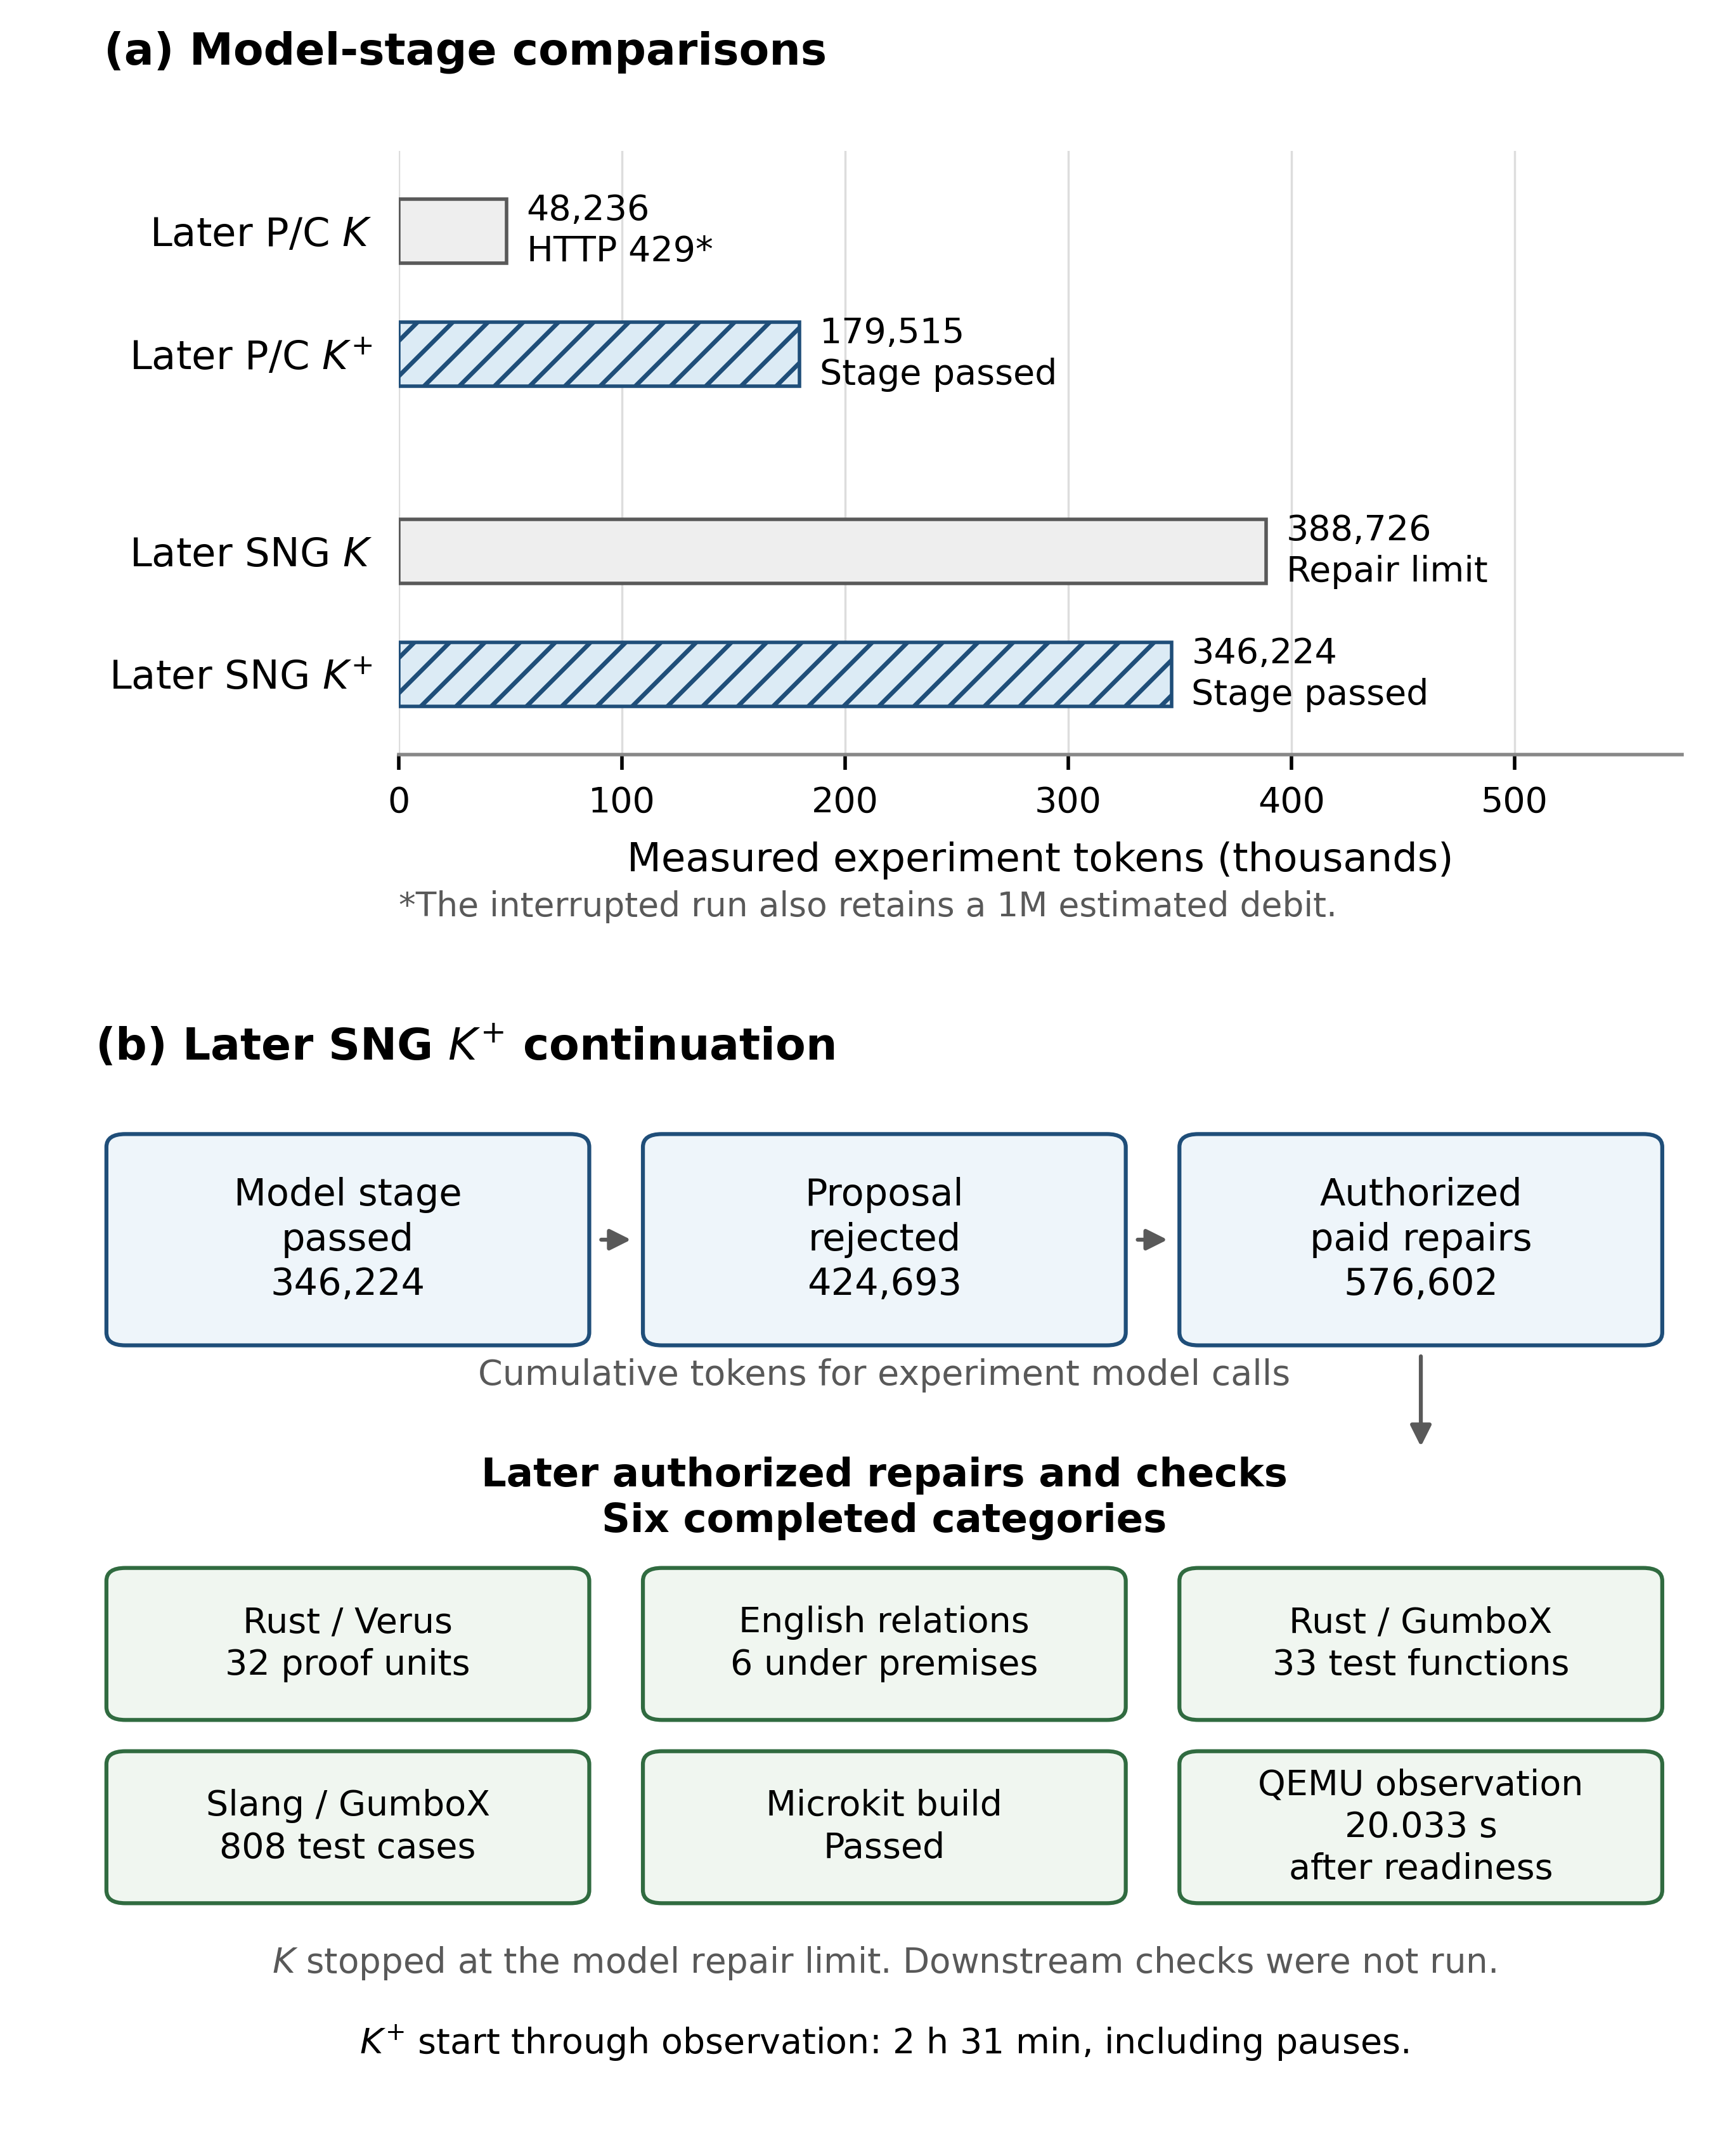
\includegraphics[width=\linewidth]{assets/comparison-results.png}
\caption{Later model comparisons for Producer/Consumer (P/C) and SNG. Panel (a) shows measured tokens through each model outcome. Panel (b) follows the later SNG $K^{+}$ candidate through the rejected proposal, paid repairs, and final checks. Serializer and initialization repairs after the paid calls add no measured experiment-model tokens. Appendix~\ref{app:evaluation-details} reports the first SNG construction separately.}
\Description{Four bars show the later Producer/Consumer K at 48236 measured tokens with HTTP 429, K plus at 179515 with one completed model target, later SNG K at 388726 at its repair limit, and later SNG K plus at 346224 with one completed model target. The continued K plus candidate used 576602 experiment-model tokens. The later SNG baseline's downstream checks were not run.}
\label{fig:comparison-results}
\end{figure}


\clearpage
\section{Requirements Review Procedure and Case Evidence}
\label{app:requirements-review}
Algorithm~\ref{alg:requirements-fidelity} details Figure~\ref{fig:requirements-review}. Campaign record $\mathcal{C}$ retains the English inputs, requirement table, candidates, costs, evidence, and decisions. Task $T$ names the reviewed scope, checks, and limits; $R$ identifies selected rule revisions. The table maps each source obligation to its interpretation, representation, assumptions, evidence, and review status.

\begin{figure}[!htbp]
\centering
% ARc-inspired staged workflow. The dashed path is proposed.
\begingroup
\hyphenpenalty=10000
\exhyphenpenalty=10000
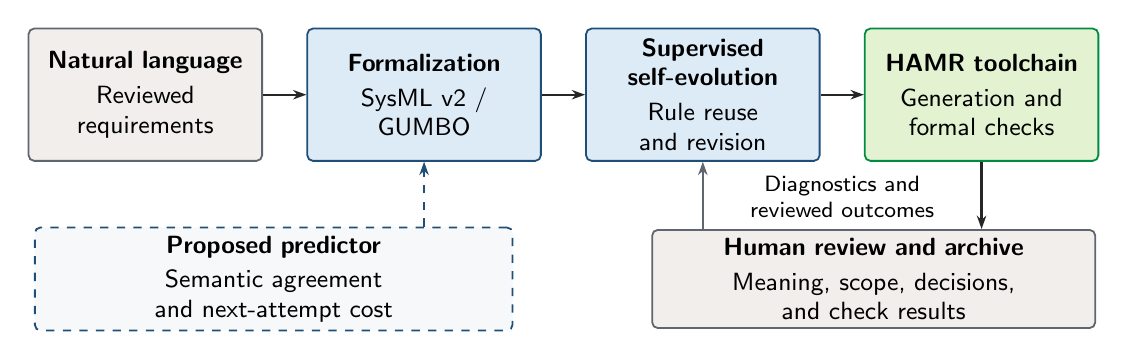
\begin{tikzpicture}[
  x=1cm,y=1cm,font=\sffamily\fontsize{9}{10.6}\selectfont,
  card/.style={rounded corners=2pt,line width=.65pt,align=center,
    text width=2.72cm,inner xsep=3.5pt,inner ysep=3pt,minimum height=1.68cm},
  support/.style={card,minimum height=1.03cm},
  flow/.style={-{Stealth[length=1.7mm,width=1.2mm]},line width=.8pt,draw=black!85},
  advisory/.style={dashed,draw=scpBlue}
]
\node[card,scpRecord] (english) at (0,0)
  {\textbf{Natural language}\\[2pt]Reviewed\\requirements};
\node[card,scpProposal] (formal) at (3.54,0)
  {\textbf{Formalization}\\[2pt]SysML v2 /\\GUMBO};
\node[card,scpProposal] (learn) at (7.08,0)
  {\textbf{Supervised\\self-evolution}\\[2pt]Rule reuse\\and revision};
\node[card,scpCheck] (hamr) at (10.62,0)
  {\textbf{HAMR toolchain}\\[2pt]Generation and\\formal checks};
\draw[flow] (english) -- (formal);
\draw[flow] (formal) -- (learn);
\draw[flow] (learn) -- (hamr);

\node[support,advisory,fill=scpBlue!4,text width=5.82cm] (predict) at (1.63,-2.34)
  {\textbf{Proposed predictor}\\[2pt]Semantic agreement and next-attempt cost};
\node[support,scpRecord,text width=5.38cm] (review) at (9.25,-2.34)
  {\textbf{Human review and archive}\\[2pt]Meaning, scope, decisions,\\and check results};
\draw[flow,advisory] (predict.north -| formal.south) -- (formal.south);
\draw[flow] (hamr.south) -- (review.north -| hamr.south);
\draw[flow,draw=scpGray] (review.north -| learn.south) -- (learn.south);
\node[align=center,font=\sffamily\fontsize{8}{9.3}\selectfont] at (8.85,-1.30)
  {Diagnostics and\\reviewed outcomes};
\end{tikzpicture}
\endgroup

\caption{From reviewed natural-language requirements to checked artifacts, inspired by ARc's formalization and feedback loop~\cite[Fig.~1, p.~4]{bayless2025arc}. Diagnostics and reviewed outcomes inform repairs and rule updates. The dashed predictor would advise which candidate to check next. Actual allowance and recorded approvals govern attempts.}
\Description{Four stages link natural-language requirements, SysML v2 and GUMBO formalization, supervised rule use and revision, and HAMR generation and formal checks. A dashed proposed predictor estimates semantic agreement and next-attempt cost. Check results flow to human review and the archive. Diagnostics and reviewed outcomes feed supervised self-evolution.}
\label{fig:requirements-review}
\end{figure}

% Intended method composition; Figure requirements-review gives the main account.
% Historical case audits and the F01 recording limitation are stated in the appendix.
\begin{algorithm}[!htbp]
\caption{Review requirements fidelity during development}
\label{alg:requirements-fidelity}
\KwIn{Campaign record $\mathcal{C}$; task $T$; selected rule revisions $R$.}
\KwOut{Updated $\mathcal{C}$ and scoped task outcome $q$.}
Retain the original English, input versions, approved scope, and rule revisions\nllabel{ln:rf-retain}\;
Read the source line by line; record obligations, interpretations, representations, and assumptions in the requirement table\;
Assess meaning and unresolved questions; record the responsible reviewer or agent\;
\lIf{$T$ lacks current human approval}{\Return \scpStatus{pending}}
\While{authority, deadline, and allowance after consumption and reservations permit an attempt}{
  \lIf{usage is unresolved}{\Return \scpStatus{pending}}
  \lIf{reviewed inputs or dependencies have changed}{\Return \scpStatus{stale}}
  Reserve allowance; request a proposal for $T$ using $R$\;
  Record usage, proposal, and detailed call outcome\;
  \lIf{response is invalid or check time is unavailable}{\Return \scpStatus{pending}}
  Run HAMR and the required checks; retain results, failures, obligation links, and content fingerprints\nllabel{ln:rf-check}\;
  Update the requirement table; review interpretation, assumptions, and unresolved obligations\;
  Apply current human decisions with Algorithm~\ref{alg:attestation}; request any required new review; obtain $q$\;
  \If{$q$ is accepted}{
    Mark the included task scope complete; record the owner's release decision when supplied, with exclusions and remaining obligations\;
    \Return $q$\;
  }
  \lIf{$q$ is stale or rejected}{\Return $q$}
  \If{the next action changes meaning, scope, assumptions, or limits}{
    Retain the proposal; \Return \scpStatus{pending} for human review\nllabel{ln:rf-amend}\;
  }
  \lIf{rule revision follows a current failed \texttt{NOT\_VALIDATED} use of the same rule and learning plan}{\Return \texttt{NOT\_VALIDATED}}
  \lIf{the next action lacks repair authority}{\Return $q$}
  Retain earlier charges and failures; refine within the approved scope and retry\;
}
\Return \scpStatus{pending} for further allowance or instruction\;
\end{algorithm}


This procedure composes development, accounting, and review services~\cite{scpCheckpoint}. The reported Producer/Consumer and SNG cases used saved source and proof audits. Their review criteria followed the start of generation; SNG's final six-relation audit followed runtime. Appendix~\ref{app:coverage-details} gives the actual mappings and service configuration.

Appendix~\ref{app:semantic-budget} describes the proposed use of predictions to select attempts. Historical engineering results retain their status; later owner release decisions record their dates and scopes.

\clearpage
\section{Early Assessment and Budgeted Search}
\label{app:semantic-budget}
An early semantic assessment asks whether a proposed interpretation is likely to preserve the source obligations and assumptions. Its prediction can guide which candidate receives the next formalization attempt. Research Preference Models motivate assessing candidates before costly execution~\cite{foster2026rpm}; reusable algorithmic structure provides a reason to expect earlier experience to help the search~\cite{e28030332}. Verification and human review then assess the resulting artifacts and their scope.

\subsection{Semantic Prediction and Its Geometry}
The workbench supplies the comparisons and forecasts in Table~\ref{tab:semantic-comparisons}~\cite{scpCheckpoint}. Automatic use of their predictions to admit attempts and rank search branches is a proposed extension. The later SNG reconstruction supplied 66 preselected entries in its $K^{+}$ input and used that set throughout. Section~\ref{sec:fidelity} describes the separate source and contract reviews.

\begin{table}[!htbp]
\caption{Comparison inputs and outputs in the inspected implementation.}
\label{tab:semantic-comparisons}
\centering\small
\begin{tabular}{@{}p{.20\linewidth}p{.43\linewidth}p{.31\linewidth}@{}}
\hline
Mechanism & Inputs & Output and use \\
\hline
Rule retrieval & Task query; rule trigger and principle & Lexical cosine distance; selects related guidance. \\
Contract comparison & Features of assumptions and guarantees after architecture assessment & Cosine distance; supports review of contract differences. \\
Model forecast & Reviewed learning material, declared task, and available feedback & Model belief score and explanation for the next application. \\
\hline
\end{tabular}
\end{table}

For rule retrieval, $x$ counts words and symbols in the task query and $y$ those in a rule's trigger and principle. Nonzero vectors satisfy the configured comparison when
\begin{equation}
d_{\cos}(x,y)=1-\frac{x\cdot y}{\|x\|\|y\|}\leq\epsilon.
\label{eq:retrieval-distance}
\end{equation}
The retrieval default is $\epsilon=0.1$, with allowed values in $[0,0.3]$. Contract comparison uses features of assumptions and guarantees after architecture checking. These representations approximate similarity: counting words and symbols gives $a\leq b$ and $b\leq a$ the same representation. A model assessment can examine the relation and explain uncertainty. A distance limit corresponds to an angle $\theta_{\max}=\arccos(1-\epsilon_{\max})$ around the reference direction.

Figure~\ref{fig:semantic-cone} retains the reference, candidate directions, and applicability boundary illustrated by Tahat et al.~\cite[slide~12]{tahat2026dascslides}. Green and check marks denote a favorable prediction that sends a candidate to formal assurance within the remaining budget. Crosses identify illustrative candidates for refinement or review. The construction extends to any specification language for which paired requirements, candidate representations, and suitable checks are defined; the engineering cases here use SysML/GUMBO. Forecast calibration is a subject for future evaluation.

\begin{figure}[!htbp]
\centering
% Vector redraw of Tahat et al., slide 12. Marks show illustrative predictions.
\begingroup
\hyphenpenalty=10000
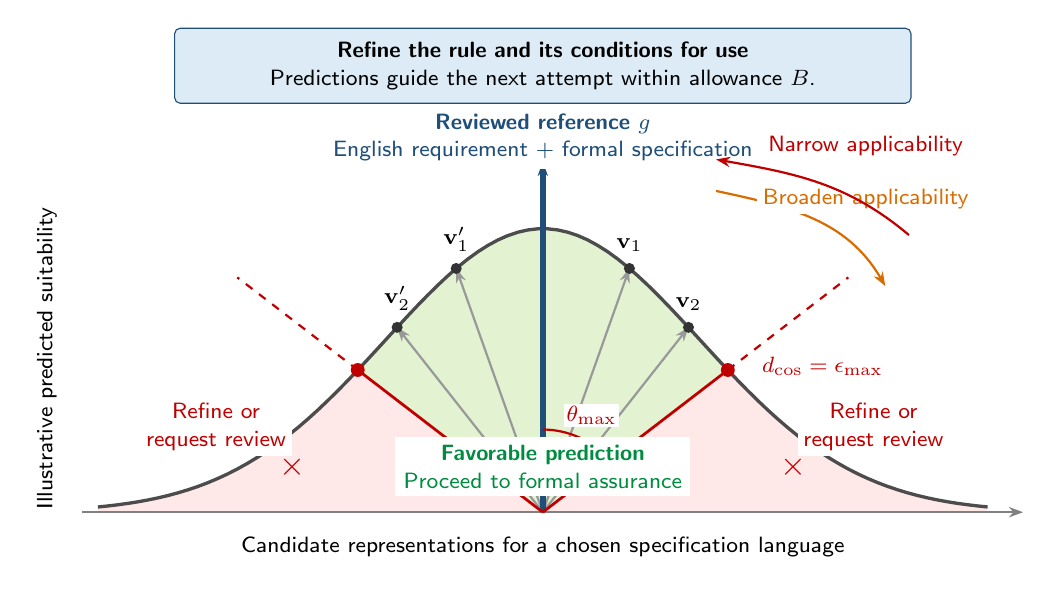
\begin{tikzpicture}[
 x=1cm,y=1cm,font=\sffamily\fontsize{8.5}{10}\selectfont,
 arrow/.style={-{Stealth[length=1.8mm,width=1.3mm]},line width=.8pt},
 note/.style={align=center,fill=white,inner sep=3pt},
 good/.style={text=scpGreen,font=\sffamily\bfseries\fontsize{12}{13}\selectfont},
 bad/.style={text=scpRed,font=\sffamily\bfseries\fontsize{12}{13}\selectfont}
]
\path[fill=scpRedFill] (.35,0) --
  plot[domain=.35:11.65,samples=90] (\x,{3.6*exp(-((\x-6)^2)/8)}) -- (11.65,0) -- cycle;
\path[fill=scpGreenFill] (6,0) --
  plot[domain=3.65:8.35,samples=50] (\x,{3.6*exp(-((\x-6)^2)/8)}) -- cycle;
\draw[arrow,draw=black!50] (.15,0) -- (12.1,0);
\node[rotate=90,align=center] at (-.30,1.95)
  {Illustrative predicted suitability};
\node[align=center] at (6,-.44)
  {Candidate representations for a chosen specification language};
\draw[black!70,line width=1.2pt,domain=.35:11.65,samples=90]
  plot (\x,{3.6*exp(-((\x-6)^2)/8)});
\foreach \x/\lab in {4.9/{\mathbf v'_1},7.1/{\mathbf v_1},4.15/{\mathbf v'_2},7.85/{\mathbf v_2}}{
  \pgfmathsetmacro{\yy}{3.6*exp(-((\x-6)^2)/8)}
  \draw[arrow,black!40] (6,0) -- (\x,\yy);
  \fill[black!80] (\x,\yy) circle (2pt);
  \node[above] at (\x,\yy+.09) {$\lab$};
}
\draw[arrow,scpBlue,line width=2pt] (6,0) -- (6,4.45);
\node[note,text=scpBlue] at (6,4.76)
  {\textbf{Reviewed reference $g$}\\English requirement + formal specification};
\foreach \x in {3.65,8.35}{
  \draw[scpRed,line width=1pt] (6,0) -- (\x,1.806);
  \fill[scpRed] (\x,1.806) circle (2.5pt);
}
\draw[scpRed,dashed,line width=.8pt] (3.65,1.806) -- (2.12,2.982);
\draw[scpRed,dashed,line width=.8pt] (8.35,1.806) -- (9.88,2.982);
\draw[arrow,scpRed] (6,1.05) arc[start angle=90,end angle=37.55,radius=1.05];
\node[note,inner sep=1pt,text=scpRed] at (6.62,1.23) {$\theta_{\max}$};
\node[note,text=scpRed,inner sep=2pt] at (9.55,1.85)
  {$d_{\cos}=\epsilon_{\max}$};
\node[good] at (5.03,2.38) {$\checkmark$};
\node[good] at (6.92,2.38) {$\checkmark$};
\node[bad] at (2.82,.57) {$\times$};
\node[bad] at (9.18,.57) {$\times$};
\node[note,text=scpGreen] at (6,.58)
  {\textbf{Favorable prediction}\\Proceed to formal assurance};
\node[note,text=scpRed,inner sep=2pt] at (1.85,1.08) {Refine or\\request review};
\node[note,text=scpRed,inner sep=2pt] at (10.2,1.08) {Refine or\\request review};
\draw[arrow,draw=orange!85!black] (8.2,4.08) to[out=-12,in=120] (10.35,2.87);
\node[note,inner sep=2pt,text=orange!85!black] at (10.1,3.98) {Broaden applicability};
\draw[arrow,draw=scpRed] (10.65,3.52) to[out=140,in=-10] (8.2,4.48);
\node[note,inner sep=2pt,text=scpRed] at (10.1,4.65) {Narrow applicability};
\node[draw=scpBlue,fill=scpBlueFill,rounded corners=2pt,
  text width=9.0cm,align=center,inner sep=5pt] at (6,5.67)
  {\textbf{Refine the rule and its conditions for use}\\
   Predictions guide the next attempt within allowance $B$.};
\end{tikzpicture}
\endgroup

\caption{Semantic prediction around a reviewed reference, redrawn from Tahat et al.~\cite[slide~12]{tahat2026dascslides}. Green and check marks indicate favorable predictions: proceed to formal assurance. Red and crosses indicate refinement or review. Positions, heights, and marks are illustrative. The geometry applies to a chosen representation in any specification language; formal checks and human decisions establish the accepted scope.}
\Description{A blue reference direction for reviewed English and a formal specification lies at the center of a bell-shaped illustration. Symmetric candidate directions lie inside and outside a distance boundary. Green checks predict suitability for the next assurance phase; red crosses request refinement or review. Arrows broaden or narrow applicability.}
\label{fig:semantic-cone}
\end{figure}

\subsection{Rule Application and Budgeted Search}
Changing $\epsilon$ broadens or narrows the similarity comparison. Revising a rule changes its conditions and procedure. Each application retains the selected version and supporting evidence.

Figure~\ref{fig:budget-tree} follows Tahat et al.~\cite[slide~7]{tahat2026dascslides} from requirements through formalization and placement to code and proof. An incorrect assumption or placement can affect several downstream artifacts. Checking an earlier choice can reveal a repair before those descendants are generated. The displayed branch counts illustrate this dependency.

\begin{figure}[!htbp]
\centering
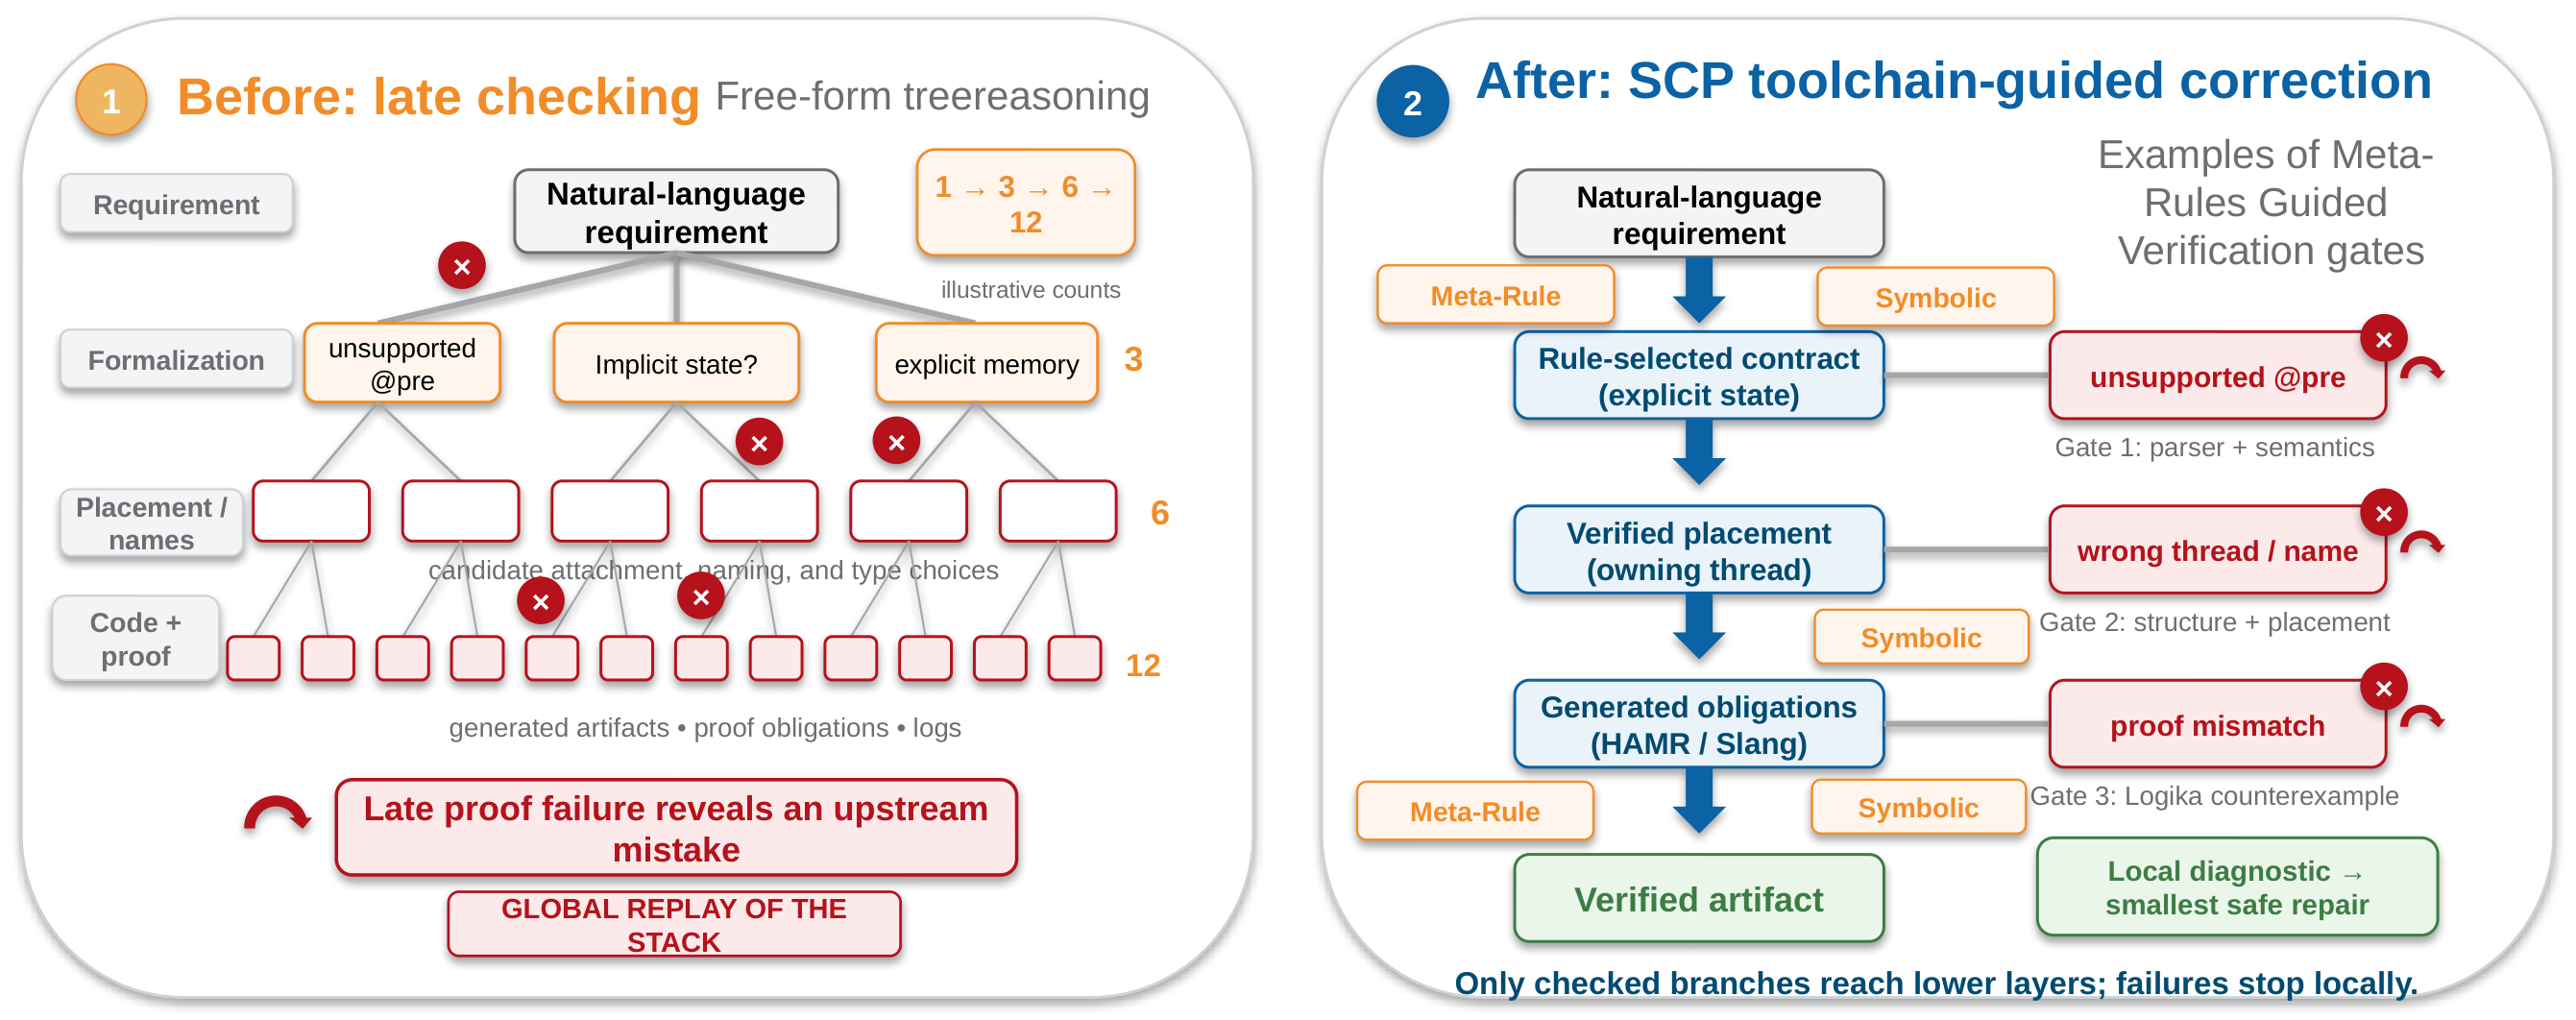
\includegraphics[width=.90\linewidth]{assets/dasc-branching-snapshot.png}
\caption{Late checking and local repair, cropped from the presentation by Tahat et al.~\cite{tahat2026dascslides}. The left panel illustrates how an early choice can multiply downstream artifacts before a failure is detected. The right panel shows checks on formalization, placement, and proof that return diagnostics at the failing stage. The branch counts are illustrative.}
\Description{The left panel is a branching tree from a requirement through formalization and placement choices to code and proof artifacts. The right panel shows a candidate contract, its placement, and proof obligations, with local repair feedback at each of three checks.}
\label{fig:branching-motivation}
\end{figure}

\begin{figure}[!htbp]
\centering
% Native vector redraw of the branching and local-check concept in Tahat et al., slide 7.
\begingroup
\hyphenpenalty=10000
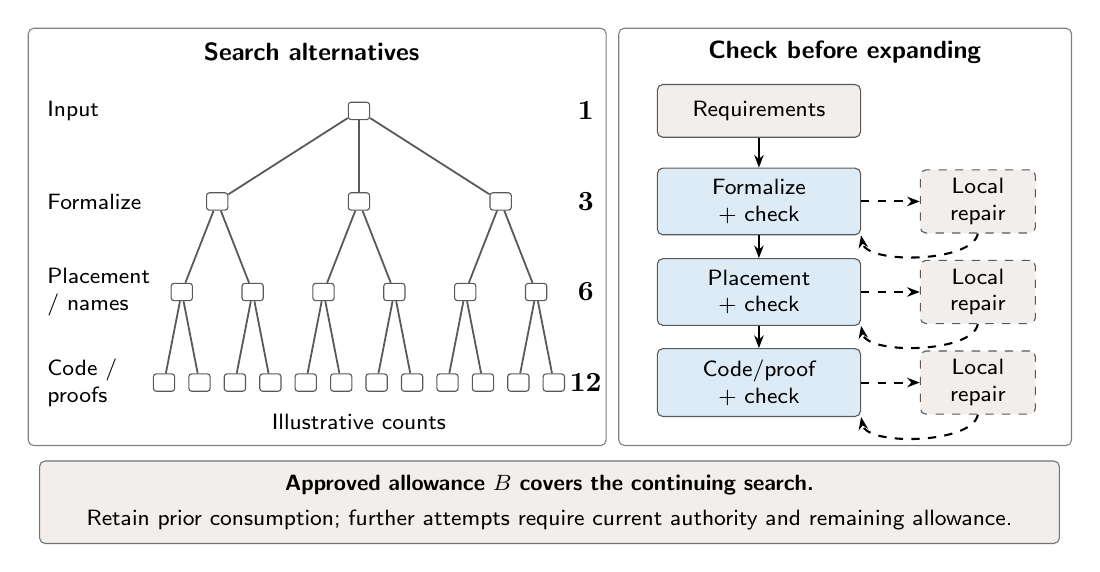
\begin{tikzpicture}[
 x=1cm,y=1cm,font=\sffamily\fontsize{8.3}{9.7}\selectfont,
 edge/.style={draw=black!65,line width=.65pt},
 flow/.style={-{Stealth[length=1.6mm,width=1.2mm]},line width=.75pt},
 branch/.style={draw=black!65,fill=white,rounded corners=1pt,
   minimum width=.27cm,minimum height=.22cm,inner sep=0pt},
 stage/.style={draw=black!65,fill=scpBlueFill,rounded corners=2pt,
   align=center,text width=2.30cm,minimum height=.67cm,inner sep=4pt},
 repair/.style={draw=black!65,dashed,fill=scpGrayFill,rounded corners=2pt,
   align=center,text width=1.25cm,minimum height=.63cm,inner sep=3pt}
]
\path[draw=black!50,rounded corners=2pt] (-.2,.10) rectangle (7.14,5.40);
\path[draw=black!50,rounded corners=2pt] (7.30,.10) rectangle (13.05,5.40);
\node[font=\sffamily\bfseries\fontsize{9}{10.4}\selectfont] at (3.4,5.10)
  {Search alternatives};
\node[font=\sffamily\bfseries\fontsize{9}{10.4}\selectfont] at (10.17,5.10)
  {Check before expanding};
\node[align=left,text width=1.3cm,anchor=west] at (-.08,4.35) {Input};
\node[align=left,text width=1.3cm,anchor=west] at (-.08,3.20) {Formalize};
\node[align=left,text width=1.3cm,anchor=west] at (-.08,2.05) {Placement / names};
\node[align=left,text width=1.3cm,anchor=west] at (-.08,.90) {Code / proofs};
\node[branch] (root) at (4,4.35) {};
\foreach \x [count=\i] in {2.2,4.0,5.8}{
  \node[branch] (f\i) at (\x,3.20) {};
  \draw[edge] (root) -- (f\i);
}
\foreach \x [count=\i] in {1.75,2.65,3.55,4.45,5.35,6.25}{
  \node[branch] (p\i) at (\x,2.05) {};
  \pgfmathtruncatemacro{\parent}{ceil(\i/2)}
  \draw[edge] (f\parent) -- (p\i);
  \node[branch] (l\i) at (\x-.225,.90) {};
  \node[branch] (r\i) at (\x+.225,.90) {};
  \draw[edge] (p\i) -- (l\i);
  \draw[edge] (p\i) -- (r\i);
}
\foreach \y/\count in {4.35/1,3.20/3,2.05/6,.90/12}
  \node[font=\bfseries] at (6.88,\y) {\count};
\node[font=\sffamily\fontsize{8}{9.2}\selectfont] at (4,.40) {Illustrative counts};
\node[stage,fill=scpGrayFill] (req) at (9.08,4.35) {Requirements};
\node[stage] (formal) at (9.08,3.20) {Formalize + check};
\node[stage] (place) at (9.08,2.05) {Placement + check};
\node[stage] (proof) at (9.08,.90) {Code/proof + check};
\draw[flow] (req) -- (formal);
\draw[flow] (formal) -- (place);
\draw[flow] (place) -- (proof);
\foreach \stageName/\stageY in {formal/3.20,place/2.05,proof/.90}{
  \node[repair] (fix-\stageName) at (11.86,\stageY) {Local repair};
  \draw[flow,dashed] (\stageName.east) -- (fix-\stageName.west);
  \draw[flow,dashed] (fix-\stageName.south) to[out=-100,in=-80,looseness=.65] (\stageName.south east);
}
\node[draw=black!55,fill=scpGrayFill,rounded corners=2pt,align=center,
  text width=12.6cm,inner sep=5pt] at (6.42,-.62)
  {\textbf{Approved allowance $B$ covers the continuing search.}\\[3pt]
   Retain prior consumption; further attempts require current authority and remaining allowance.};
\end{tikzpicture}
\endgroup

\caption{Illustrative search and local repair, redrawn from Tahat et al.~\cite[slide~7]{tahat2026dascslides}. The $1\rightarrow3\rightarrow6\rightarrow12$ expansion shows possible branching. Checks can stop an unsuitable choice and return diagnostics to the stage that produced it. These counts describe the illustration; the experiments report their actual attempts and consumption separately.}
\Description{The left tree grows from one requirement to three formalizations, six placement choices, and twelve code or proof branches. The right path checks formalization, placement, and proof choices as they arise, with local repair loops. One approved allowance covers earlier and future attempts.}
\label{fig:budget-tree}
\end{figure}

\paragraph{Proposed agreement and cost prediction}
For a requirement and candidate under stated premises, an agreement model could learn from human review outcomes, using the on-demand forecast and contract-feature similarity as inputs. A cost model could estimate incremental wall time and model tokens from attempts with comparable artifact sizes, check plans, and tool versions. Candidate ordering would favor likely agreement within the remaining time and token allowance. Estimates with sparse supporting records would carry uncertainty and could trigger review. Linking predictions to observed costs and review outcomes would let us evaluate calibration and saved effort.

Further attempts require current authority, an unexpired deadline, and available allowance after recorded consumption and outstanding reservations. Unresolved usage blocks further model calls. A stopped branch retains its attempted artifacts, diagnostics, and charges. An implementation repair can continue within current authority; a change to requirements, assumptions, scope, or limits returns to human review. A current failed use of the same rule and learning plan can supply feedback for rule revision. An authorized extension preserves earlier consumption across the continuing campaign.

\clearpage
\section{Requirement Coverage and Evidence Links}
\label{app:coverage-details}
\suppressfloats[t]

This appendix supports the fidelity claims in Section~\ref{sec:fidelity}. The anonymous extract \path{evidence/coverage-method-audit.json} records the selected source identifiers, full SHA-256 fingerprints, and evidence links. Its service-source fingerprints match the SNG study freeze. The extract contains selected facts; the complete execution archive remains separate~\cite{scpCheckpoint,sngFinalReport2026}.

Producer/Consumer and SNG retain requirement mappings in case-specific audit tables linked to their source, contract, and check records. Table~\ref{tab:sng-requirement-trace} follows one relation in the SNG audit. The campaign records also retain attempts, resource use, assumptions, and review decisions.

\begin{table}[!htbp]
\caption{One recorded SNG requirement-to-evidence trace. Identifiers refer to the accompanying extract.}
\label{tab:sng-requirement-trace}
\centering\small
\begin{tabular}{@{}p{.17\linewidth}p{.78\linewidth}@{}}
\hline
Link & Recorded contents \\
\hline
English & \texttt{Req\_R\_2.a}: a Restricted payload above 100 becomes 100 (E1, line 38). \\
Model & The named guarantee \path{Req_R_2_a_Clamp_Above_100} occurs in the software model (M1, line 90). \\
Contracts & Gate preserves the Restricted message; Filter requires the present Restricted output to contain 100 (C1, C2). \\
Evidence & Saved Gate and Filter crate proofs pass. Audit A1 links the contracts to the checked compute methods (P1, P2). \\
Review & Approval H1 covers the initialization premise and repair. The component relation passes under its premises. \texttt{POWERUSERS-1} approved release of the recorded engineering scope on 8 November; system occurrence correspondence remains a separate obligation. \\
\hline
\end{tabular}
\end{table}

The example assumes empty outgoing slots at dispatch entry and relies on generated external input/output interfaces. The approved initialization premise has supporting factory/composition proofs; correspondence with the actual wrapper and physical transport remains unresolved. The audit retains these limits alongside the passing component relation.

The P1 and P2 proof receipts bind their respective Rust application files, C1 and C2. Their recorded SHA-256 fingerprints match the corresponding entries in the build and observation inventories in \path{evidence/evidence-audit.json}. These matches identify the application files across checks and builds. The separate runtime evidence measures boot and receiver liveness.

The controller fingerprints declared input-file bytes and resolved configuration. Stored records are rechecked against their hashes; architecture records also identify the tool and comparison procedure. Review fingerprints cover evidence, scope, exclusions, and blockers. Comparing these values during retrieval or a protected action detects changed contents. The linked proposal, check, and decision records identify the responsible agent or human for each reviewed version.

Human review remains explicit for non-behavioral requirements, including timing and deployment, and for assumptions or exclusions. An exclusion records its reason, revisit condition, and approval against the assessed evidence; acceptance requires current passing included checks and current approval. Technical claims still require the applicable analysis, proof, test, or observation. For this SNG case, timing guarantees and full system correspondence remain open.

The workbench also provides optional structured requirement-mapping and proof-unit services. Their configuration fields, \texttt{requirement\_ledger} and \texttt{unit\_registry}, are unset in the inspected PC/SNG model runs; these cases use the audit tables described above. A mapping result records whether an element is located. A proof-unit result additionally binds the run, configuration, input files, unit, and checked element. The accompanying extract preserves these implementation details for reproduction.

\clearpage
\section{Review and Retrieval in the Interface}
\label{app:interface-details}
\suppressfloats[t]
\subsection{Campaign Archive and Review Interface}
\label{sec:interface}
\label{sec:retrieval}
The browser and command-line interface retrieve checks, evidence, and decisions from the same persistent campaign archive~\cite{scpCheckpoint}. From a run, an engineer can locate the failed check, verify the evidence fingerprint, and follow links to the reviewer, rationale, and decision time. The examples below show an approved scope change, the retained failure, and the corresponding retrieval commands.


\paragraph{Earlier budget authorization}
\label{sec:review-example}
\label{sec:budget-example}
The earlier 14M campaign allowance provides a concrete authorization example. Its request asks: ``Approve 60 minutes and up to 2M accounted tokens within the existing 14M ceiling, retaining prior charges and the documented best-effort/1M unmetered-failure debit policy?'' The requested 2M allowance remains within the cumulative 14M ceiling. If $u$ tokens are already accounted for, full use requires $u+2\mathrm{M}\leq14\mathrm{M}$; reservations further reduce the available balance.

The \texttt{Campaign} service records extensions against the prior allowance or deadline and preserves consumption. The 1M debit estimates usage when measurement is unavailable. Approval must be recorded separately from this request. The recorded name attributes approval; identity authentication remains external to this record~\cite{scpCheckpoint}.

\paragraph{Scope review}
In the synthetic case in Figure~\ref{fig:ui-approval-summary}, A passed and B failed. Approving B's exclusion enabled partial acceptance while retaining the failure, rationale, revisit condition, and option to revoke it. The excluded obligation receives no verification credit. The interface's separate \emph{Defer selected} action keeps B required.

\begin{figure}[!htbp]
\centering
% Print-sized excerpts from the same unedited application capture.
\begingroup
\setlength{\fboxsep}{4pt}
\setlength{\fboxrule}{0.4pt}
\fcolorbox{black!35}{black!3}{%
\begin{minipage}{\dimexpr\linewidth-2\fboxsep-2\fboxrule\relax}
\small\color{black}
\textbf{(a) Verification status and evidence link}
\par\vspace{2pt}
\centering
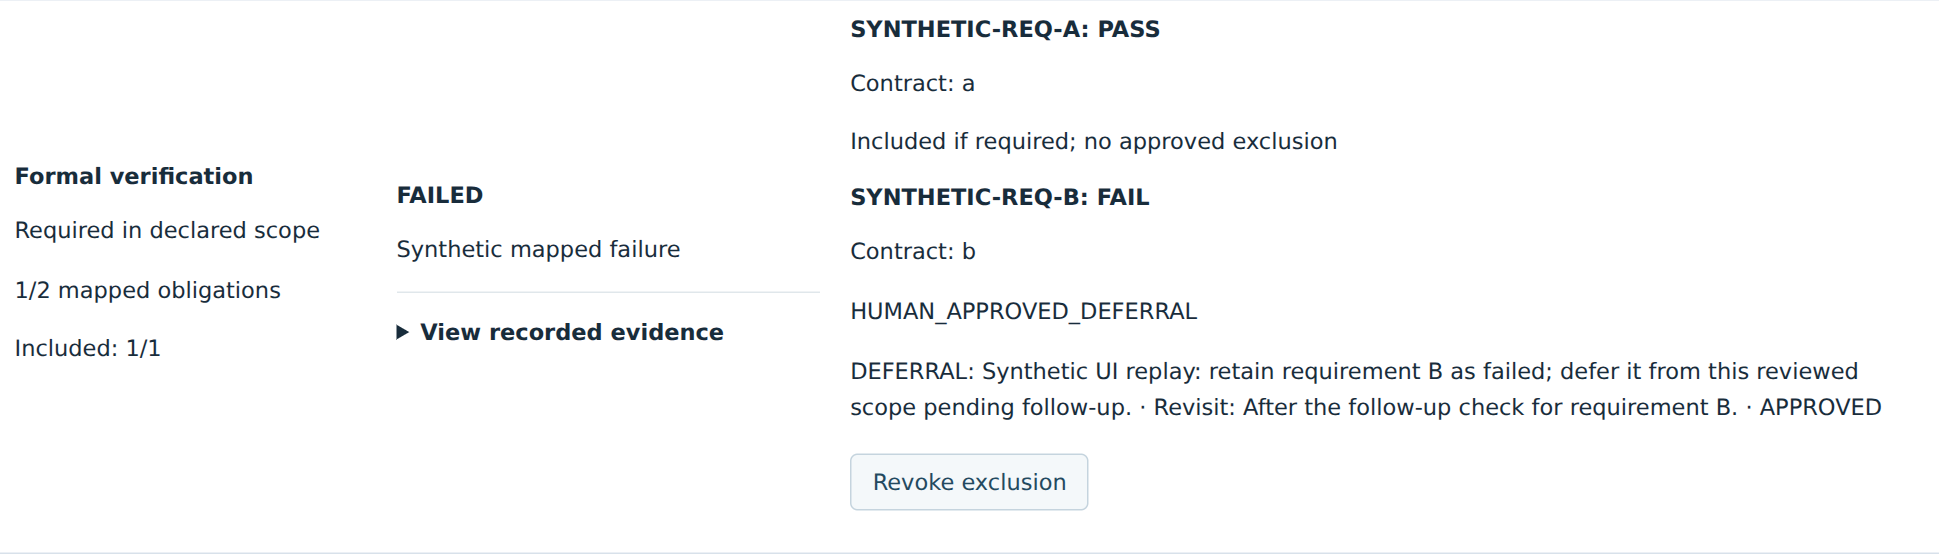
\includegraphics[width=.82\linewidth,trim=0bp 170bp 1115bp 150bp,clip]{assets/ui-approval-accepted.png}
\par\vspace{5pt}
\raggedright
\textbf{(b) Per-requirement results and approval}
\par\vspace{2pt}
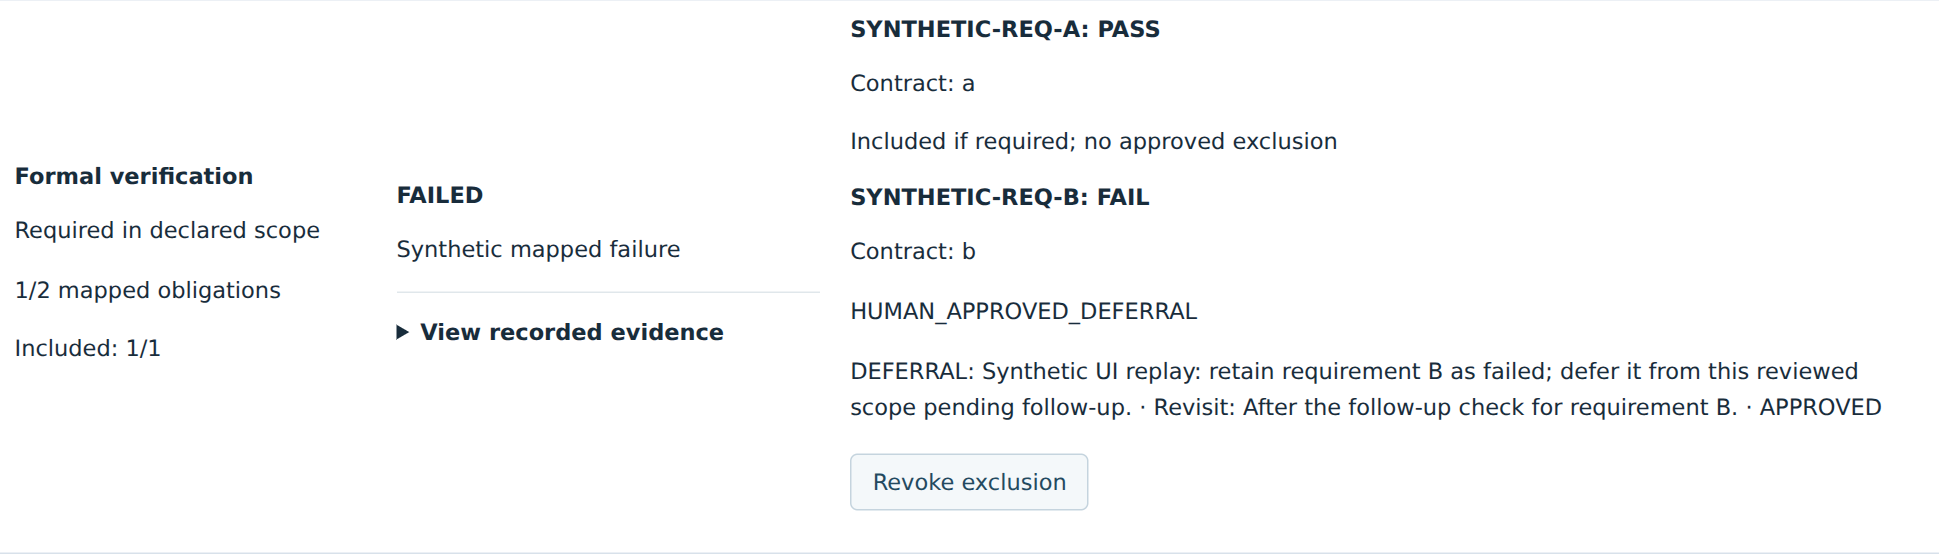
\includegraphics[width=\linewidth,trim=830bp 31bp 10bp 0bp,clip]{assets/ui-approval-accepted.png}
\end{minipage}%
}
\endgroup

\caption{Review of a synthetic case in the workbench. An approved exclusion leaves one passing obligation in scope (1/1). The original result still shows a failure and 1/2 mapped obligations. The review panel retains the rationale and revisit condition. The evidence link opens the original result.}
\Description{Two excerpts from the browser interface. The verification summary shows a failed check, one of two mapped obligations, one of one included obligations, and an evidence link. The review panel shows A passing and B failing with a human-approved exclusion, its rationale and revisit condition, and a revoke control.}
\label{fig:ui-approval-summary}
\end{figure}

\subsection{Retrieval Commands}
For that case, let $R$ be run \texttt{a83f146e}\ldots, $H$ evidence fingerprint \texttt{3db914d832ff}\ldots, and $P$ request \texttt{610bd646}\ldots. With \texttt{./scp-workbench --state-dir STATE}, the schematic queries are
\begin{quote}\small\ttfamily
trace R\\
trace R --evidence H\\
approval P
\end{quote}
The trace identifies the failed check and $H$. The second query retrieves the A-pass/B-fail evidence and checks its SHA-256. The review record links it to B's exclusion and request $P$; the third query retrieves approval, reviewer label, and decision time. A separate acceptance record binds the review fingerprint. The original trace remains \texttt{FAILED}.

Signed export uses a bundle location and the expected policy and trusted keys. Three pilot cases check retention across clean service reopening (Section~\ref{sec:evaluation}); browser-restart behavior remains untested~\cite{scpCheckpoint}.

\end{document}
